\section{Exercises}

%__________________
\subsection{Line fitting, residuals, and correlation}

% 1

\eoce{\qt{Visualize the residuals\label{visualize_residuals}} The scatterplots 
shown below each have a superimposed regression line. If we were to construct a 
residual plot (residuals versus $x$) for each, describe what those plots would 
look like.
\begin{center}
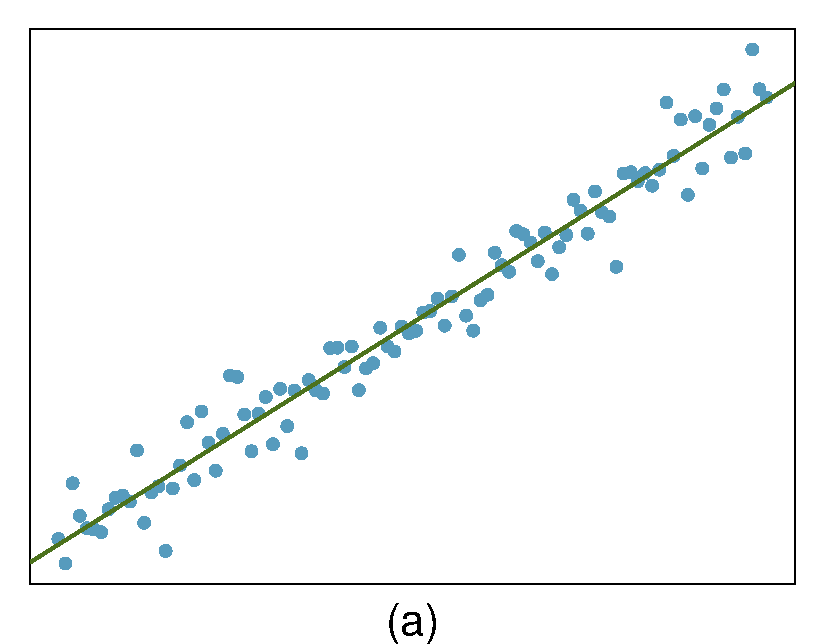
\includegraphics[width=0.42\textwidth]{ch_regr_simple_linear/figures/eoce/visualize_residuals/visualize_residuals_linear.pdf} 
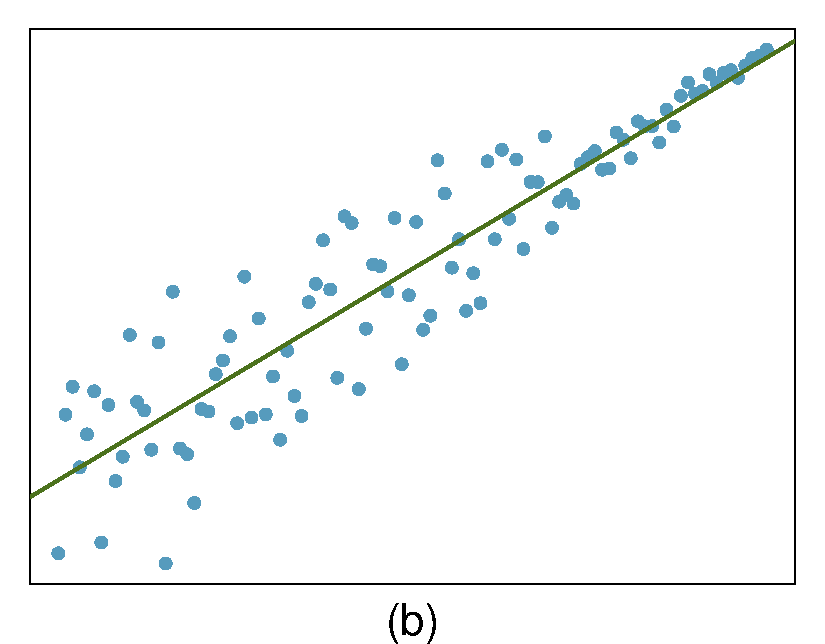
\includegraphics[width=0.42\textwidth]{ch_regr_simple_linear/figures/eoce/visualize_residuals/visualize_residuals_fan_back.pdf}
\end{center}
}{}

% 2

\eoce{\qt{Trends in the residuals\label{trends_in_residuals}} Shown below are two 
plots of residuals remaining after fitting a linear model to two different sets 
of data. Describe important features and determine if a linear model would be 
appropriate for these data. Explain your reasoning.
\begin{center}
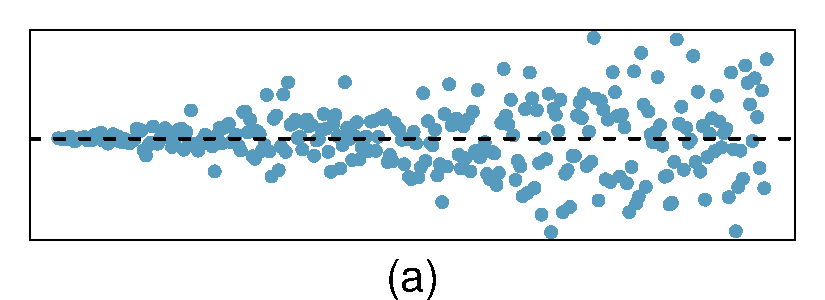
\includegraphics[width=0.42\textwidth]{ch_regr_simple_linear/figures/eoce/trends_in_residuals/trends_in_residuals_fan.pdf} 
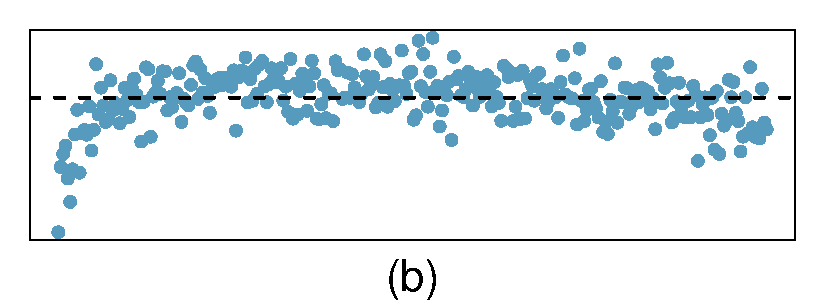
\includegraphics[width=0.42\textwidth]{ch_regr_simple_linear/figures/eoce/trends_in_residuals/trends_in_residuals_log.pdf}
\end{center}
}{}

% 3

\eoce{\qt{Identify relationships, Part I\label{identify_relationships_1}} For 
each of the six plots, identify the strength of the relationship (e.g. weak, 
moderate, or strong) in the data and whether fitting a linear model would be 
reasonable.
\begin{center}
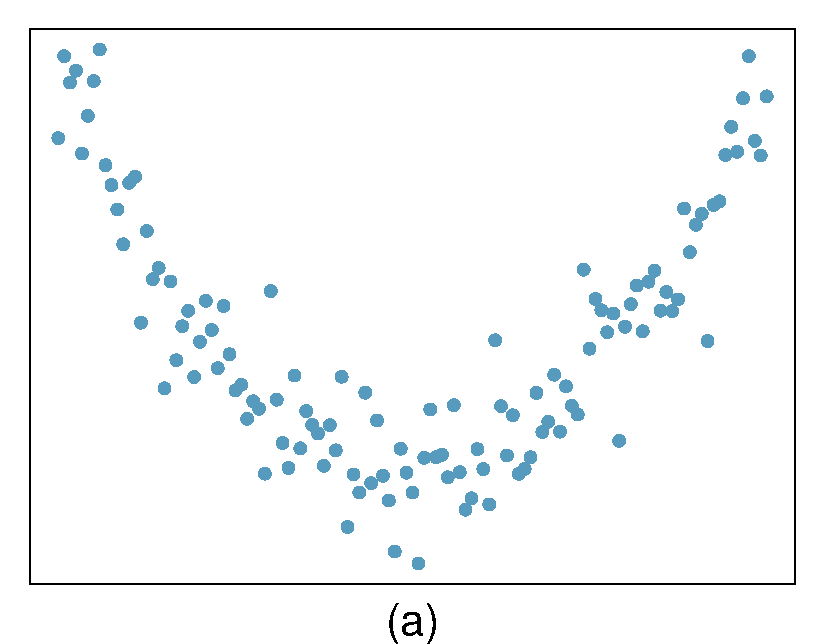
\includegraphics[width=0.32\textwidth]{ch_regr_simple_linear/figures/eoce/identify_relationships_1/identify_relationships_u.pdf}
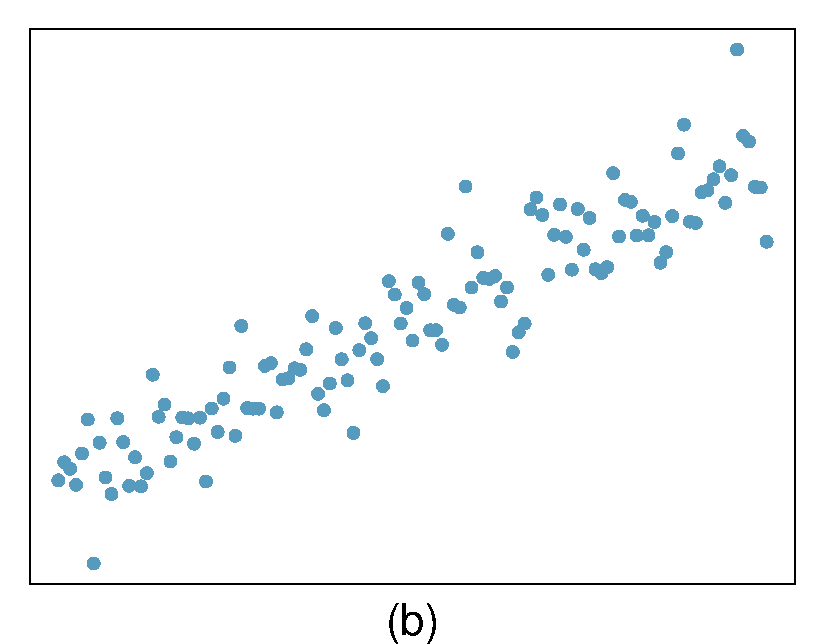
\includegraphics[width=0.32\textwidth]{ch_regr_simple_linear/figures/eoce/identify_relationships_1/identify_relationships_lin_pos_strong.pdf}
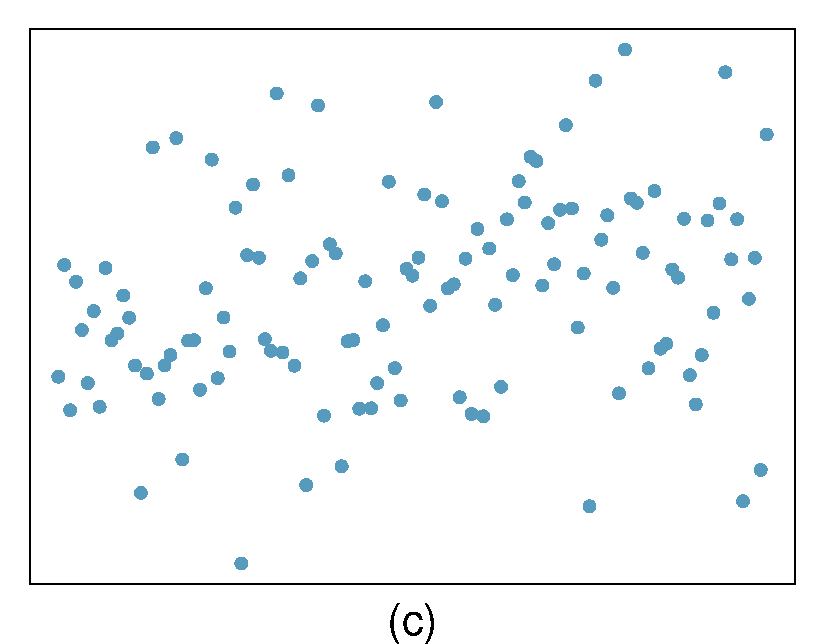
\includegraphics[width=0.32\textwidth]{ch_regr_simple_linear/figures/eoce/identify_relationships_1/identify_relationships_lin_pos_weak.pdf}
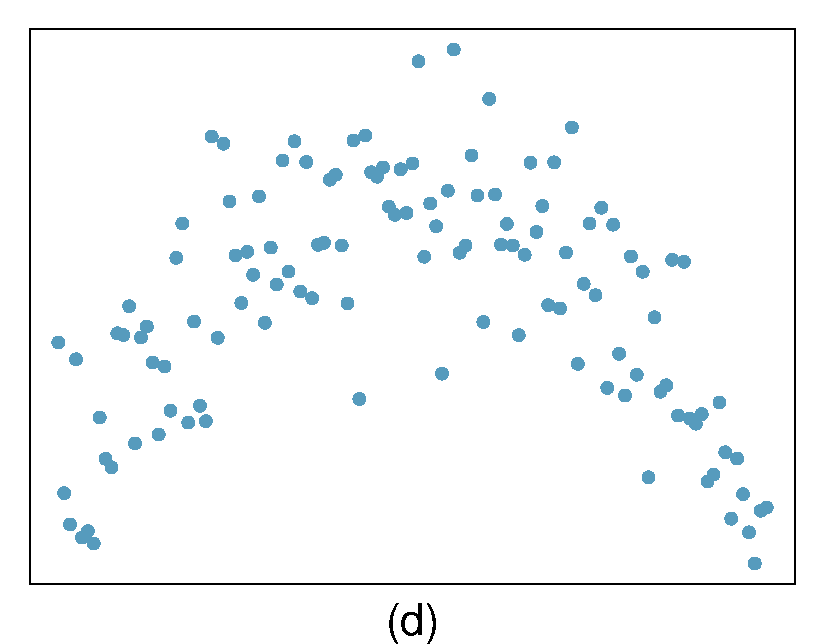
\includegraphics[width=0.32\textwidth]{ch_regr_simple_linear/figures/eoce/identify_relationships_1/identify_relationships_n.pdf}
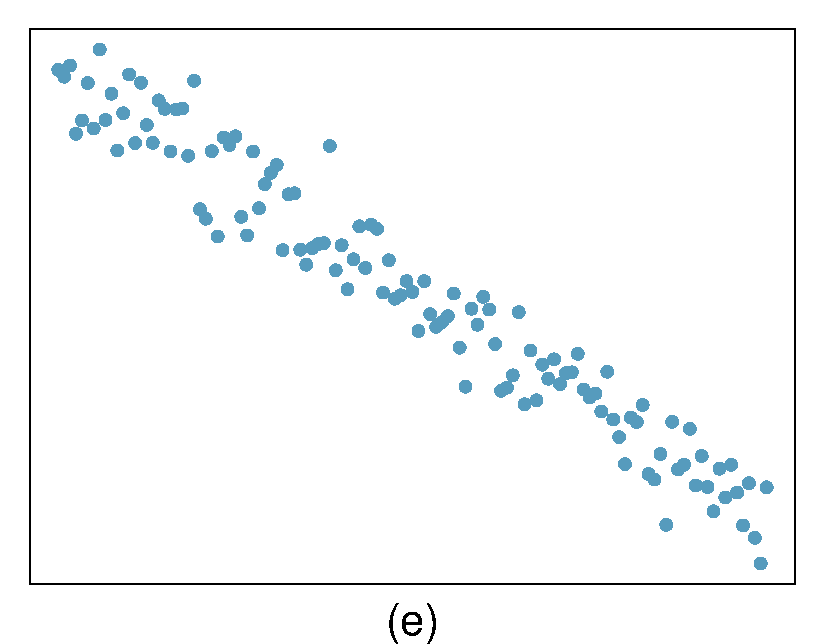
\includegraphics[width=0.32\textwidth]{ch_regr_simple_linear/figures/eoce/identify_relationships_1/identify_relationships_lin_neg_strong.pdf}
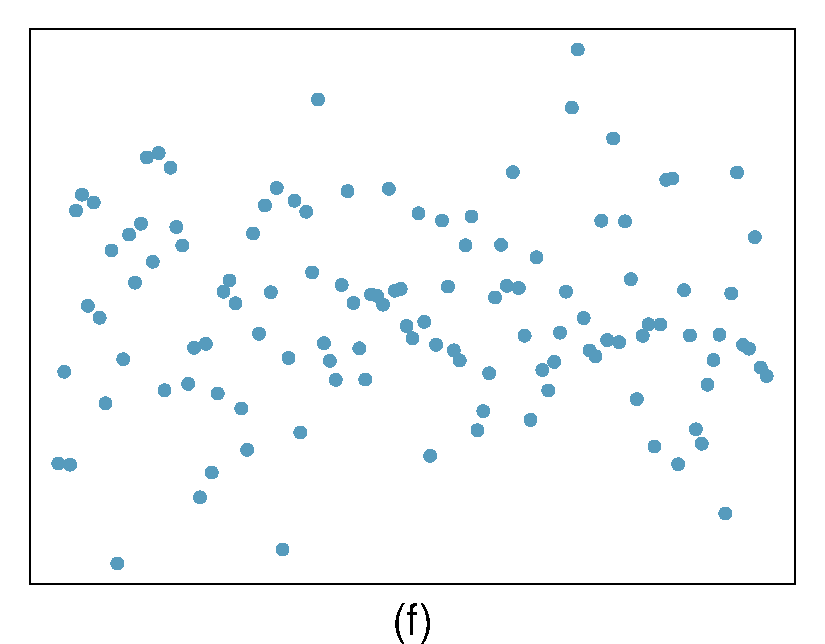
\includegraphics[width=0.32\textwidth]{ch_regr_simple_linear/figures/eoce/identify_relationships_1/identify_relationships_none.pdf}
\end{center}
}{}

% 4

\eoce{\qt{Identify relationships, Part II\label{identify_relationships_2}} For 
each of the six plots, identify the strength of the relationship (e.g. weak, 
moderate, or strong) in the data and whether fitting a linear model would be 
reasonable.
\begin{center}
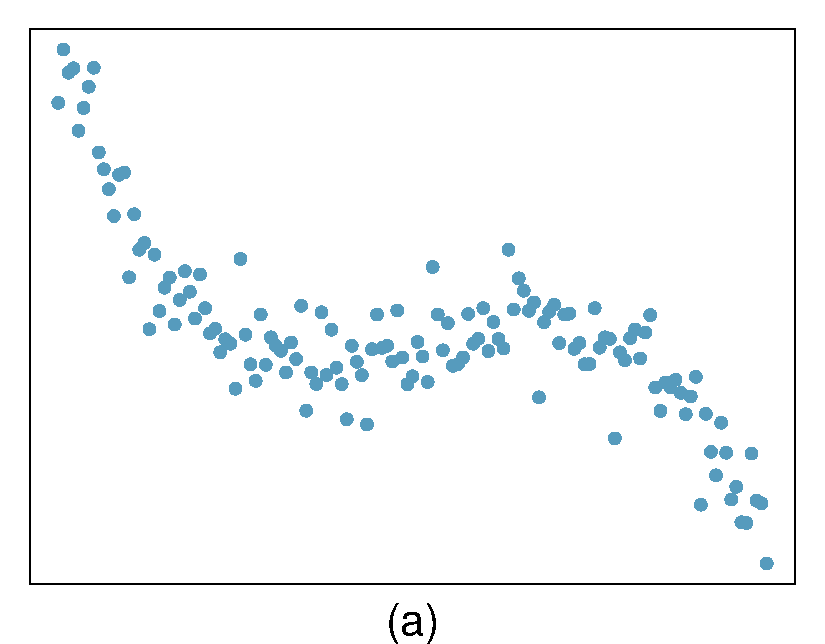
\includegraphics[width=0.32\textwidth]{ch_regr_simple_linear/figures/eoce/identify_relationships_2/identify_relationships_s.pdf}
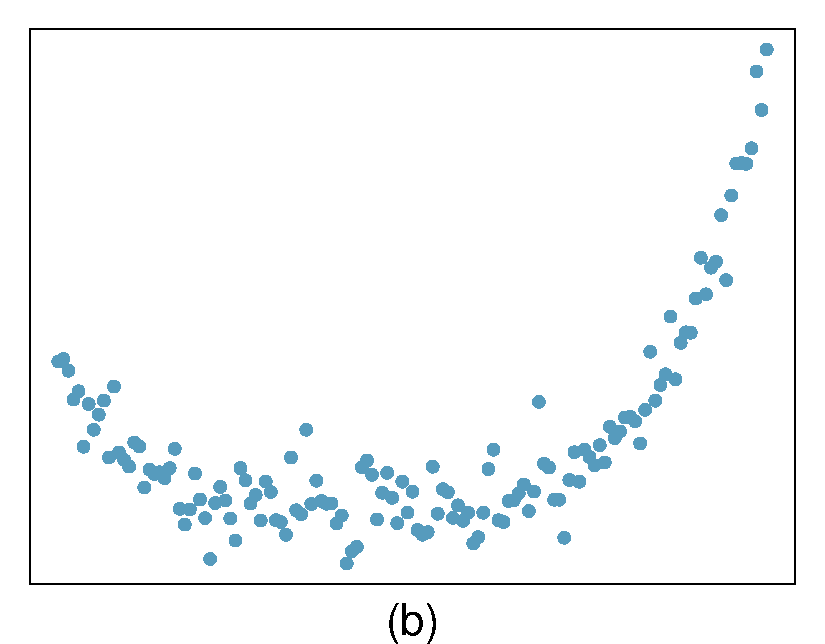
\includegraphics[width=0.32\textwidth]{ch_regr_simple_linear/figures/eoce/identify_relationships_2/identify_relationships_hockey_stick.pdf}
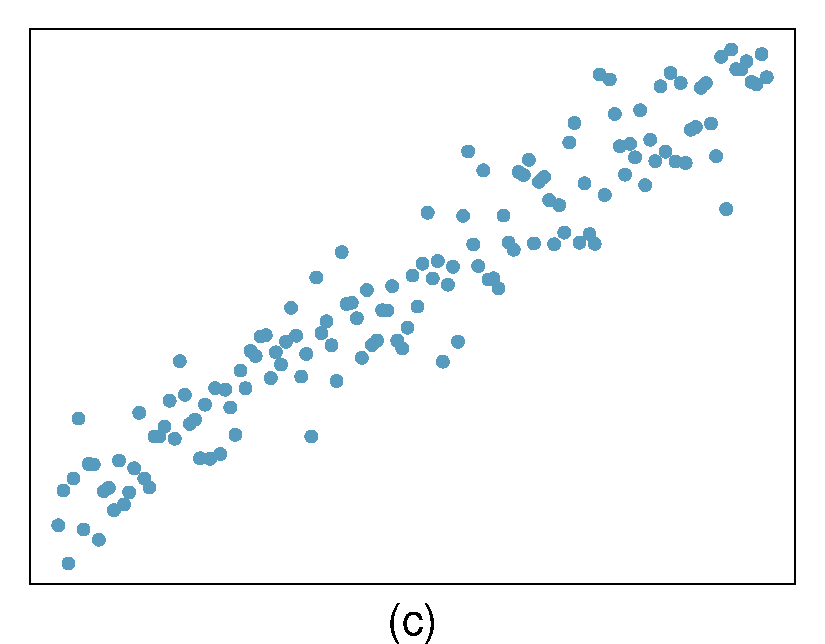
\includegraphics[width=0.32\textwidth]{ch_regr_simple_linear/figures/eoce/identify_relationships_2/identify_relationships_pos_lin_strong.pdf}
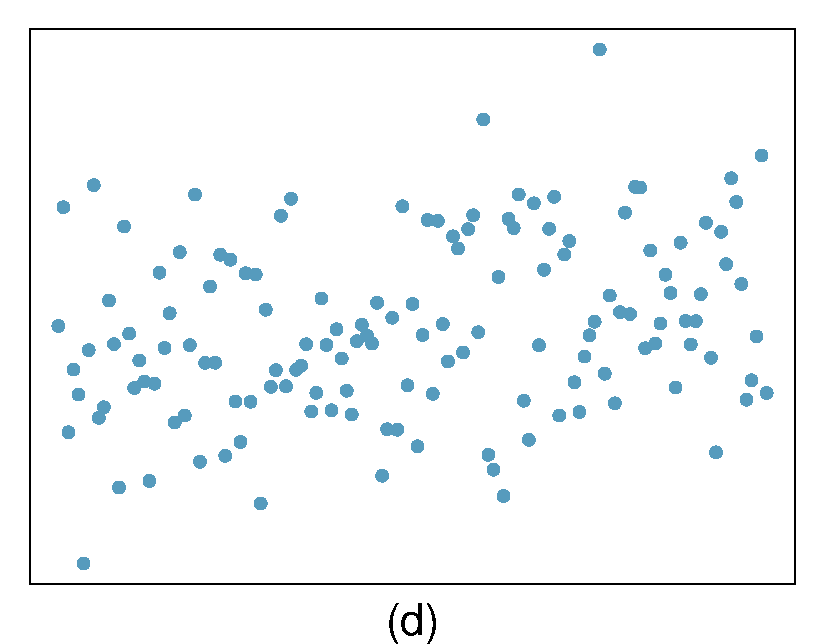
\includegraphics[width=0.32\textwidth]{ch_regr_simple_linear/figures/eoce/identify_relationships_2/identify_relationships_pos_weak.pdf}
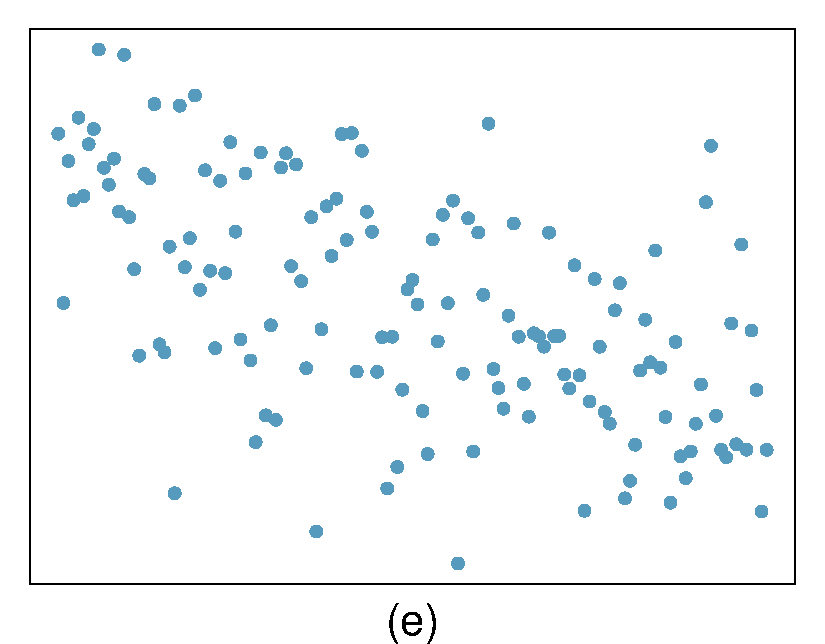
\includegraphics[width=0.32\textwidth]{ch_regr_simple_linear/figures/eoce/identify_relationships_2/identify_relationships_pos_weaker.pdf}
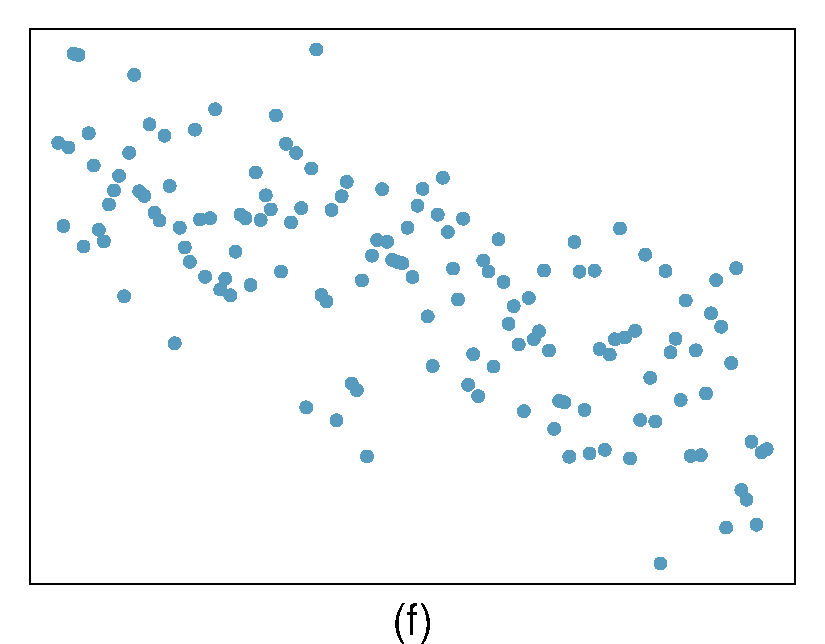
\includegraphics[width=0.32\textwidth]{ch_regr_simple_linear/figures/eoce/identify_relationships_2/identify_relationships_neg_lin_weak.pdf}
\end{center}
}{}

% 5

\eoce{\qt{Exams and grades\label{exams_grades_correlation}} The two scatterplots 
below show the relationship between final and mid-semester exam grades recorded 
during several years for a Statistics course at a university.
\begin{parts}
\item Based on these graphs, which of the two exams has the strongest correlation 
with the final exam grade? Explain.
\item Can you think of a reason why the correlation between the exam you chose in 
part (a) and the final exam is higher?
\end{parts}
\begin{center}
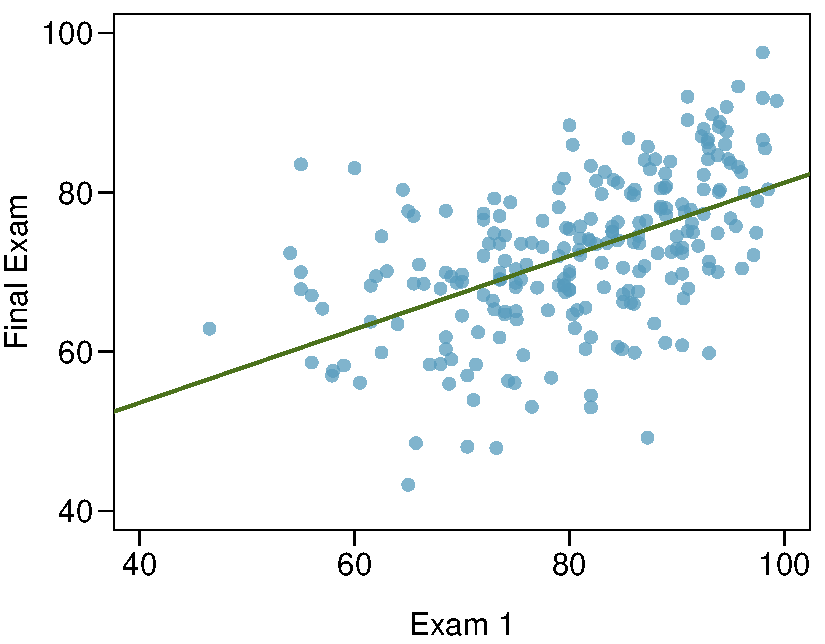
\includegraphics[width=0.49\textwidth]{ch_regr_simple_linear/figures/eoce/exams_grades_correlation/exam_grades_1.pdf}\ \ 
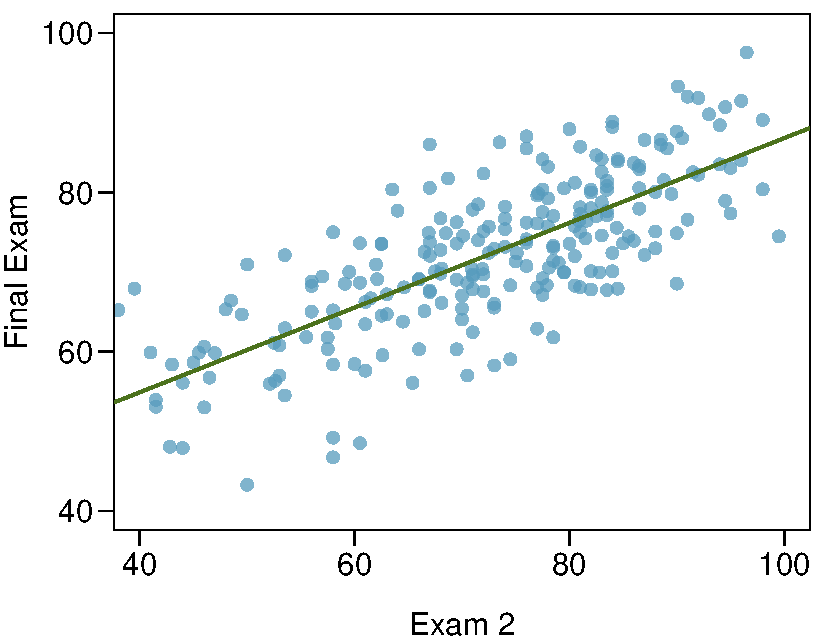
\includegraphics[width=0.49\textwidth]{ch_regr_simple_linear/figures/eoce/exams_grades_correlation/exam_grades_2.pdf}
\end{center}
}{}

% 6

\eoce{\qt{Husbands and wives, Part I\label{husbands_wives_correlation}} The Great 
Britain Office of Population Census and Surveys once collected data on a random 
sample of 170 married couples in Britain, recording the age (in years) and 
heights (converted here to inches) of the husbands and 
wives.\footfullcite{Hand:1994} The scatterplot on the left shows the wife's age 
plotted against her husband's age, and the plot on the right shows wife's height 
plotted against husband's height.
\begin{center}
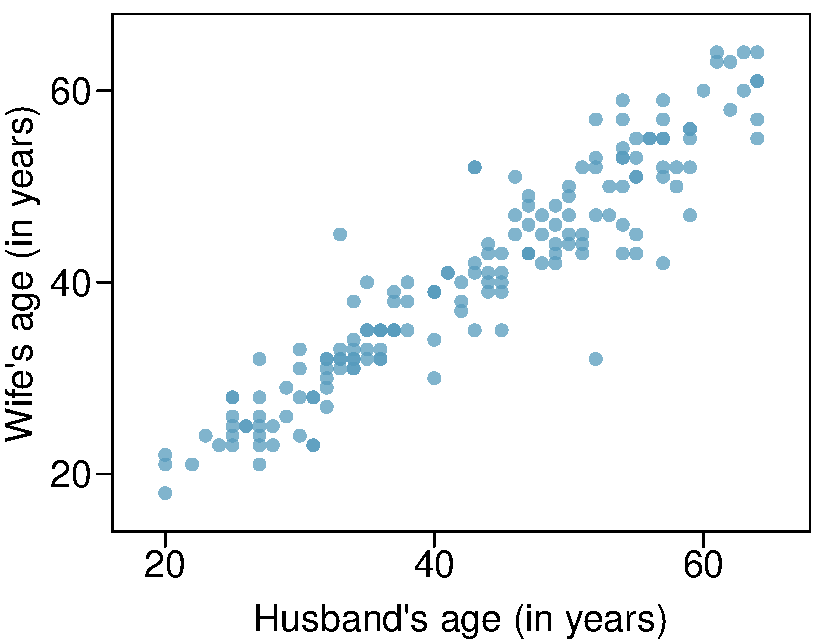
\includegraphics[width=0.38\textwidth]{ch_regr_simple_linear/figures/eoce/husbands_wives_correlation/husbands_wives_age.pdf} \hspace{5mm}
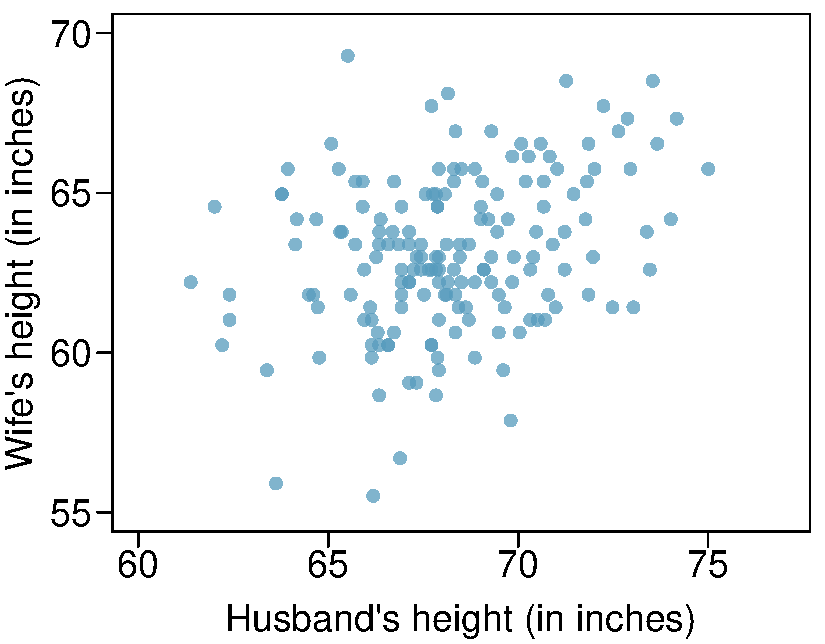
\includegraphics[width=0.38\textwidth]{ch_regr_simple_linear/figures/eoce/husbands_wives_correlation/husbands_wives_height.pdf}
\end{center}
\begin{parts}
\item Describe the relationship between husbands' and wives' ages.
\item Describe the relationship between husbands' and wives' heights.
\item Which plot shows a stronger correlation? Explain your reasoning.
\item Data on heights were originally collected in centimeters, and then 
converted to inches. Does this conversion affect the correlation between 
husbands' and wives' heights?
\end{parts}
}{}

% 7

\noindent \begin{minipage}[c]{0.43\textwidth}
\eoce{\qt{Match the correlation, Part I\label{match_corr_1}} Match the calculated 
correlations to the corresponding scatterplot.
\begin{parts}
\item $r = -0.7$
\item $r = 0.45$ 
\item $r = 0.06$
\item $r = 0.92$
\end{parts} \vspace{21mm}
}{}
\end{minipage}
\begin{minipage}[c]{0.57\textwidth}
\begin{center}
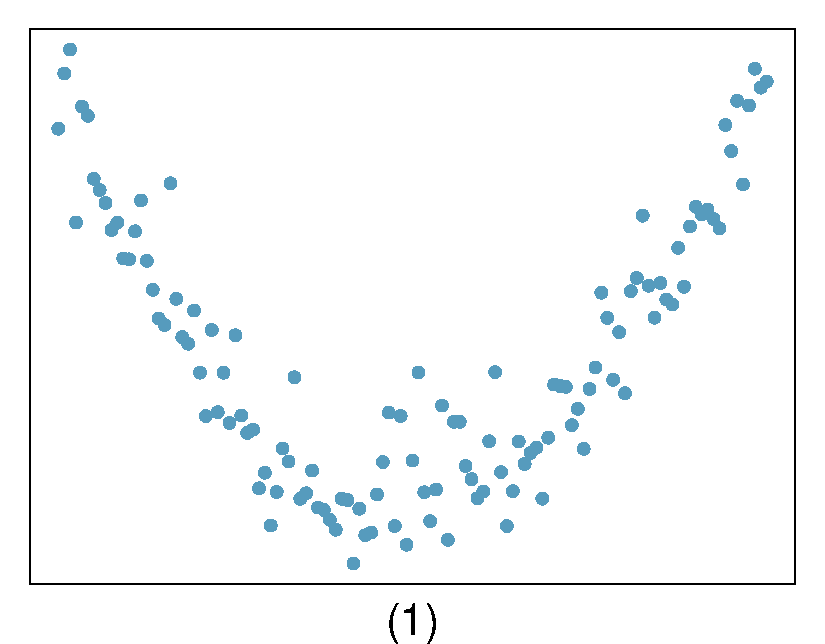
\includegraphics[width=0.45\textwidth]{ch_regr_simple_linear/figures/eoce/match_corr_1/match_corr_1_u.pdf}
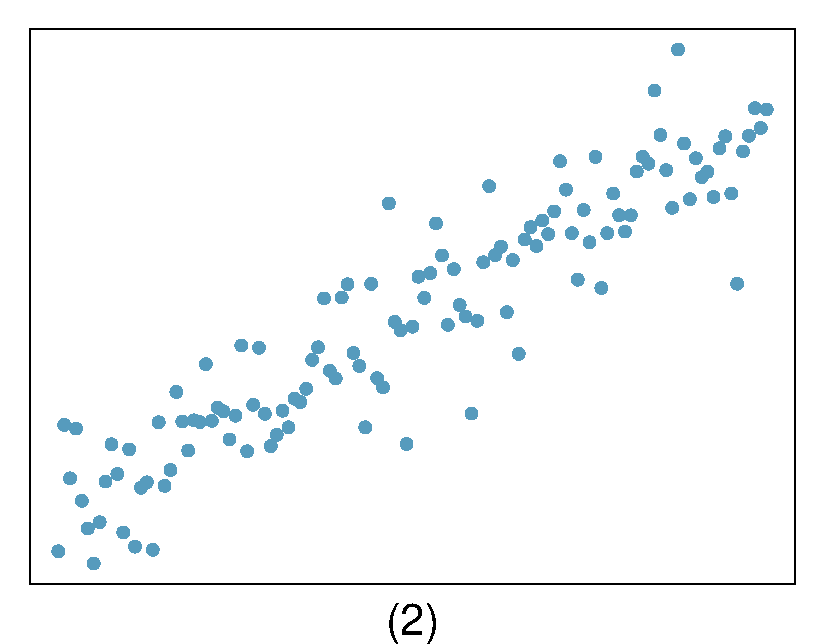
\includegraphics[width=0.45\textwidth]{ch_regr_simple_linear/figures/eoce/match_corr_1/match_corr_2_strong_pos.pdf} \\
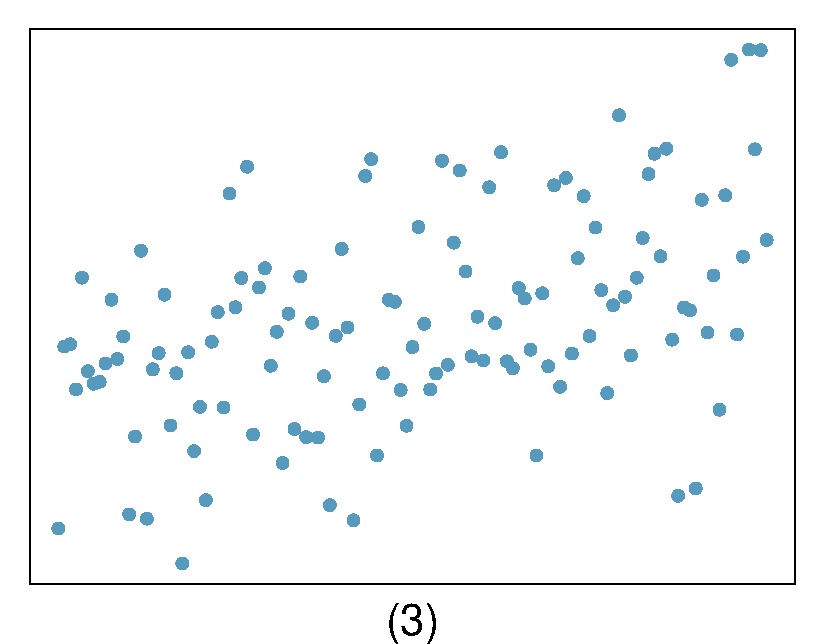
\includegraphics[width=0.45\textwidth]{ch_regr_simple_linear/figures/eoce/match_corr_1/match_corr_3_weak_pos.pdf}
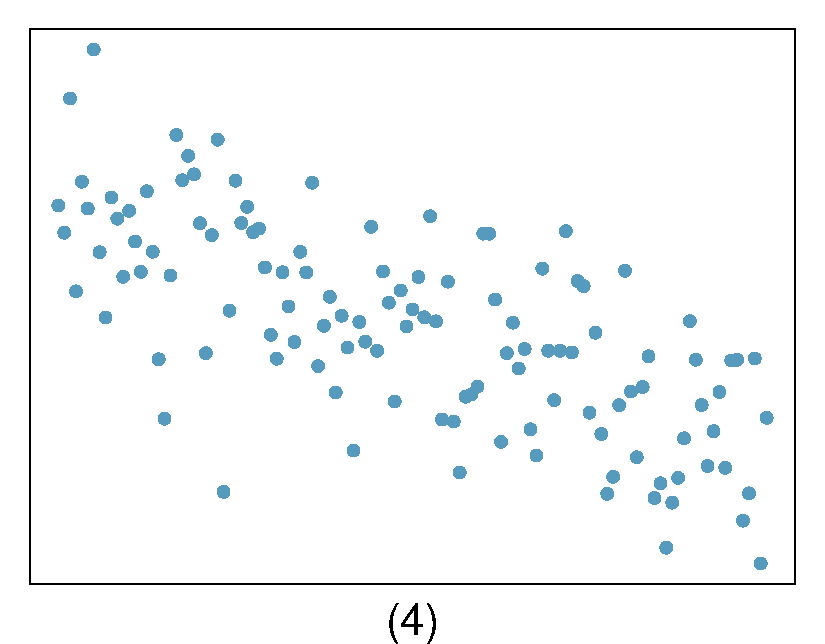
\includegraphics[width=0.45\textwidth]{ch_regr_simple_linear/figures/eoce/match_corr_1/match_corr_4_weak_neg.pdf}
\end{center}
\end{minipage}

% 8

\noindent \begin{minipage}[c]{0.43\textwidth}
\eoce{\qt{Match the correlation, Part II\label{match_corr_2}} Match the 
calculated correlations to the corresponding scatterplot.
\begin{parts}
\item $r = 0.49$
\item $r = -0.48$ 
\item $r = -0.03$ 
\item $r = -0.85$
\end{parts} \vspace{21mm}
}{}
\end{minipage}
\begin{minipage}[c]{0.57\textwidth}
\begin{center}
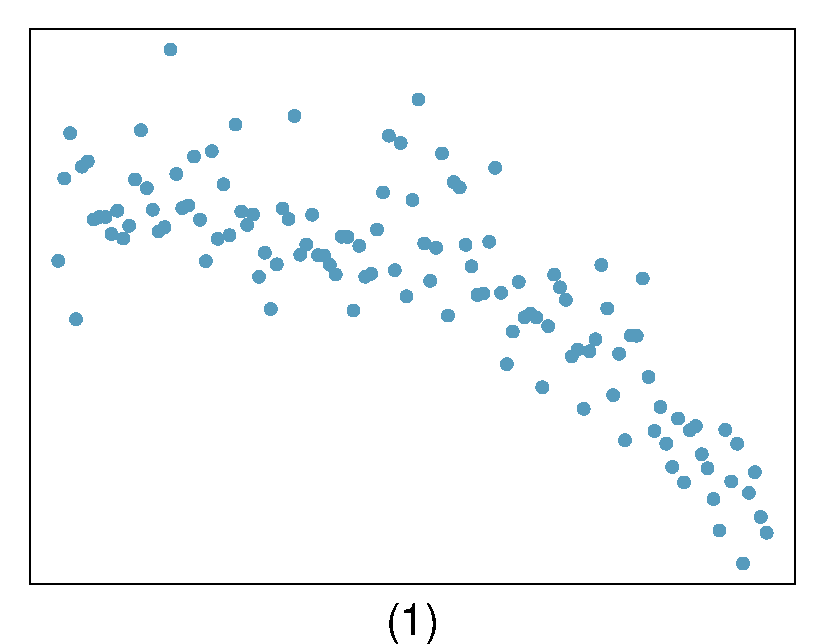
\includegraphics[width=0.45\textwidth]{ch_regr_simple_linear/figures/eoce/match_corr_2/match_corr_1_strong_neg_curved.pdf}
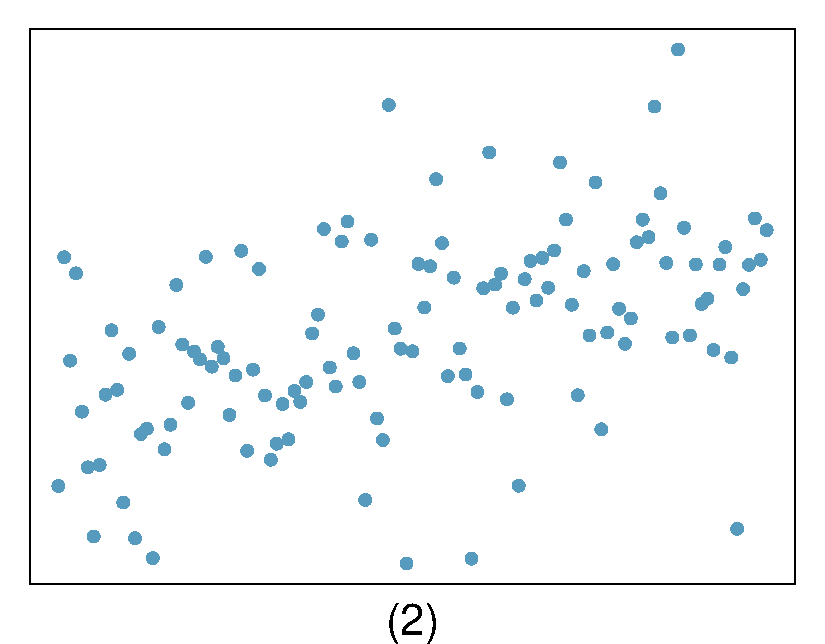
\includegraphics[width= 0.45\textwidth]{ch_regr_simple_linear/figures/eoce/match_corr_2/match_corr_2_weak_pos.pdf} \\
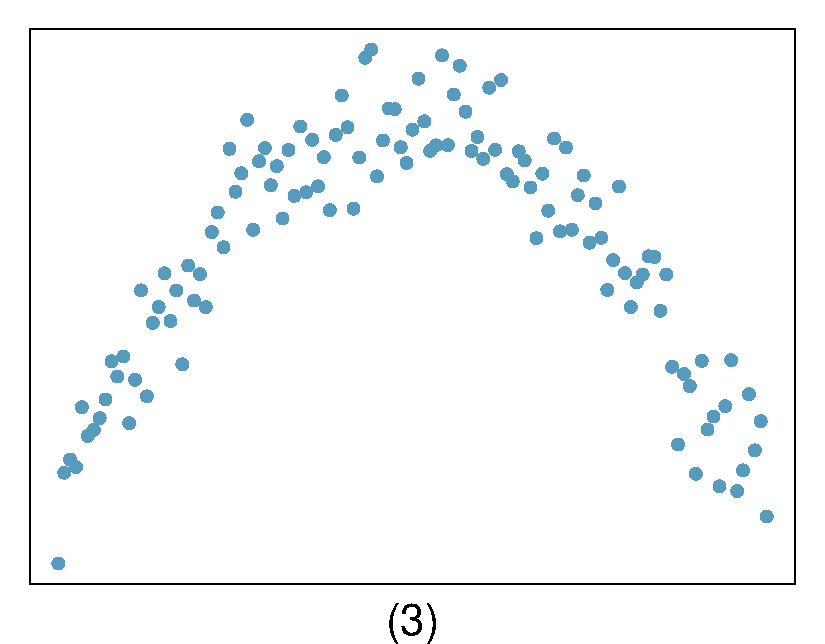
\includegraphics[width= 0.45\textwidth]{ch_regr_simple_linear/figures/eoce/match_corr_2/match_corr_3_n.pdf}
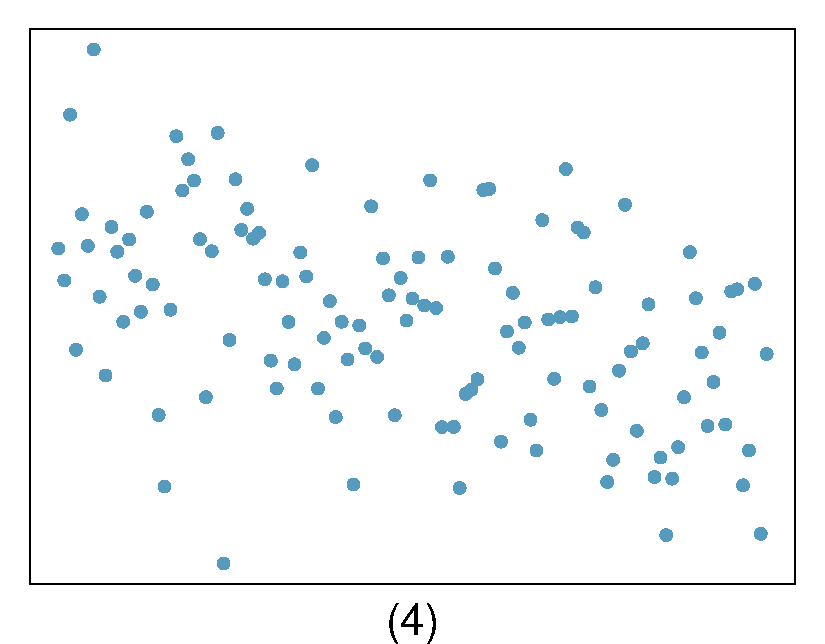
\includegraphics[width= 0.45\textwidth]{ch_regr_simple_linear/figures/eoce/match_corr_2/match_corr_4_weak_neg.pdf}
\end{center}
\end{minipage}

% 9
\eoce{\qt{True / False\label{tf_correlation}} Determine if the following 
statements are true or false. If false, explain why.
\begin{parts}
\item A correlation coefficient of -0.90 indicates a stronger linear relationship 
than a correlation coefficient of 0.5.
\item Correlation is a measure of the association between any two variables.
\end{parts}
}{}


% 10

\eoce{\qt{Guess the correlation\label{guess_correlation}} Eduardo and Rosie are 
both collecting data on number of rainy days in a year and the total rainfall for 
the year. Eduardo records rainfall in inches and Rosie in centimeters. How will 
their correlation coefficients compare?
}{}

% 11

\eoce{\qt{Speed and height\label{speed_height_gender}} 1,302 UCLA students were 
asked to fill out a survey where they were asked about their height, fastest 
speed they have ever driven, and gender. The scatterplot on the left displays the 
relationship between height and fastest speed, and the scatterplot on the right 
displays the breakdown by gender in this relationship.
\begin{center}
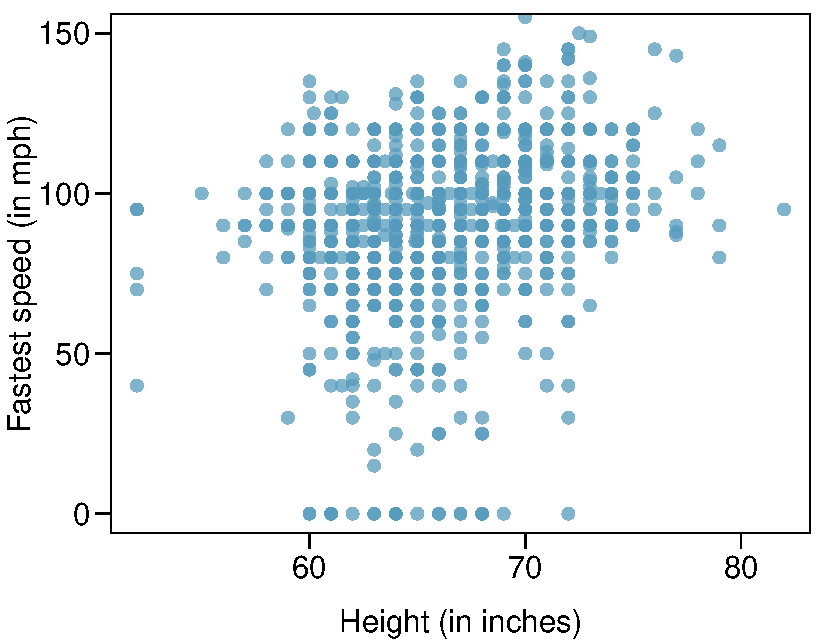
\includegraphics[width=0.485\textwidth]{ch_regr_simple_linear/figures/eoce/speed_height_gender/speed_height.pdf}\hspace{0.02\textwidth}%
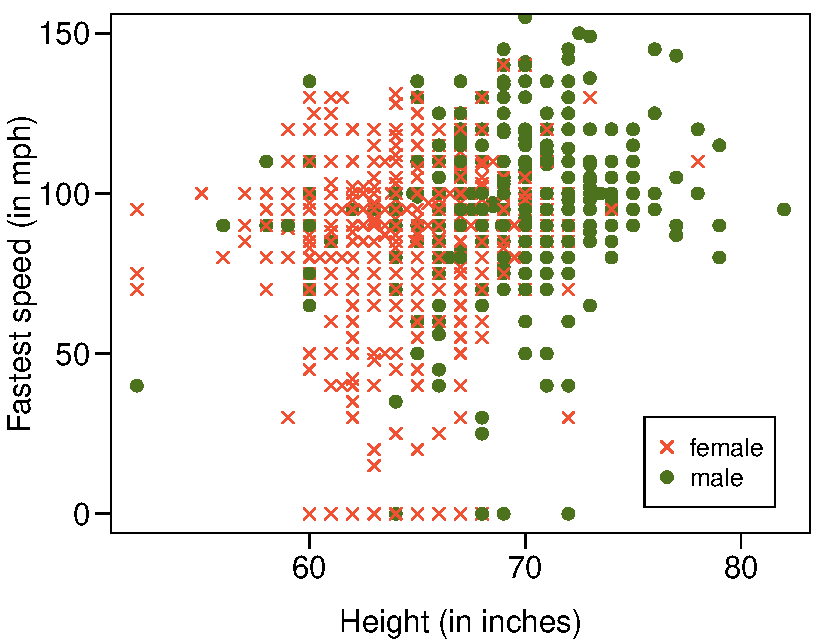
\includegraphics[width=0.485\textwidth]{ch_regr_simple_linear/figures/eoce/speed_height_gender/speed_height_gender.pdf}
\end{center}
\begin{parts}
\item Describe the relationship between height and fastest speed.
\item Why do you think these variables are positively associated?
\item What role does gender play in the relationship between height and fastest 
driving speed?
\end{parts}
}{}

% 12

\eoce{\qt{Trees\label{trees_volume_height_diameter}} The scatterplots below show 
the relationship between height, diameter, and volume of timber in 31 felled 
black cherry trees. The diameter of the tree is measured 4.5 feet above the 
ground.\footfullcite{data:trees}
\begin{center}
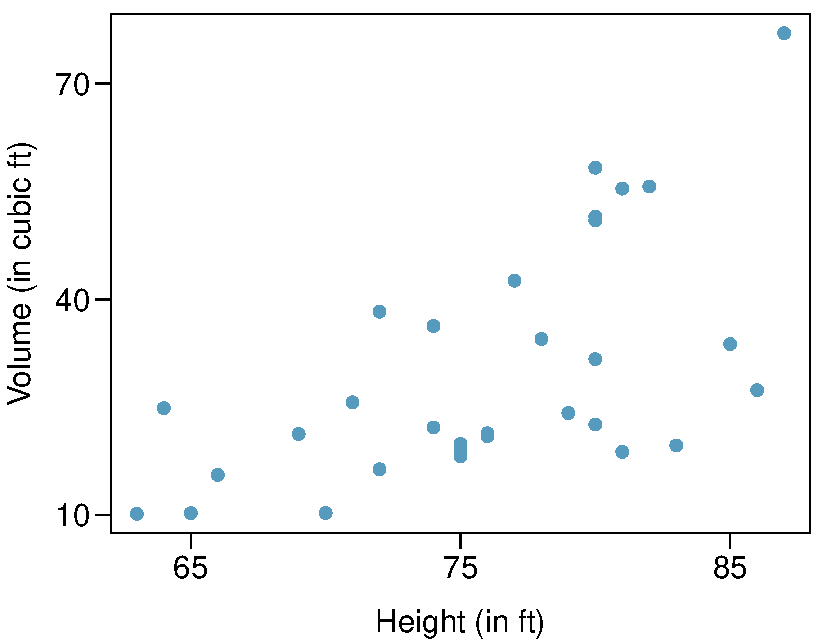
\includegraphics[width=0.485\textwidth]{ch_regr_simple_linear/figures/eoce/trees_volume_height_diameter/trees_volume_height.pdf}\hspace{0.02\textwidth}%
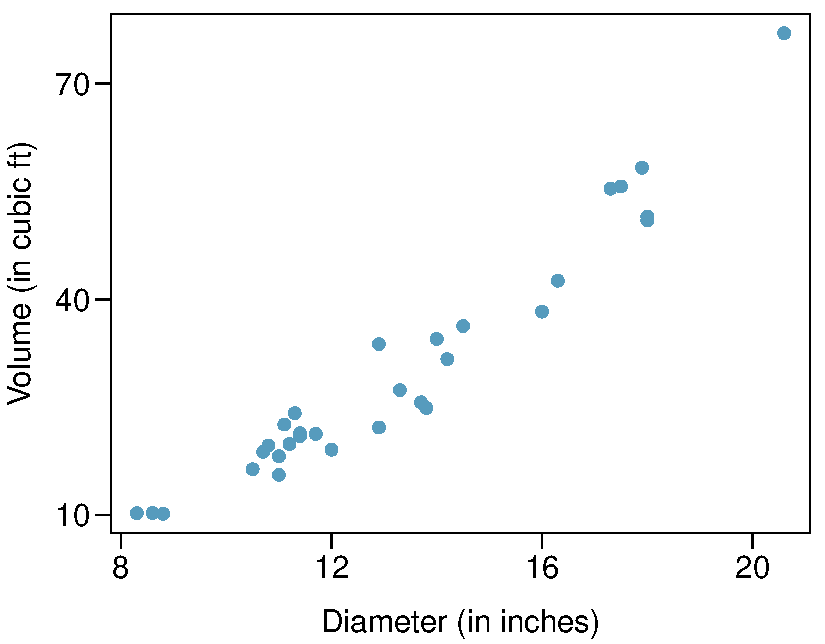
\includegraphics[width=0.485\textwidth]{ch_regr_simple_linear/figures/eoce/trees_volume_height_diameter/trees_volume_diameter.pdf}
\end{center}
\begin{parts}
\item Describe the relationship between volume and height of these trees.
\item Describe the relationship between volume and diameter of these trees.
\item Suppose you have height and diameter measurements for another black cherry 
tree. Which of these variables would be preferable to use to predict the volume 
of timber in this tree using a simple linear regression model? Explain your 
reasoning.
\end{parts}
}{}

% 13

\eoce{\qt{The Coast Starlight, Part I\label{coast_starlight_corr_units}} The 
Coast Starlight Amtrak train runs from Seattle to Los Angeles. The scatterplot 
below displays the distance between each stop (in miles) and the amount of time 
it takes to travel from one stop to another (in minutes).\vspace{2mm}

\noindent\begin{minipage}[c]{0.4\textwidth}
\begin{parts}
\item Describe the relationship between distance and travel time.
\item How would the relationship change if travel time was instead measured in 
hours, and distance was instead measured in kilometers?
\item Correlation between travel time (in miles) and distance (in minutes) is 
$r = 0.636$. What is the correlation between travel time (in kilometers) and 
distance (in hours)?
\end{parts} \vspace{7mm}
\end{minipage}
\begin{minipage}[c]{0.05\textwidth}
$\:$\\
\end{minipage}
\begin{minipage}[c]{0.52\textwidth}
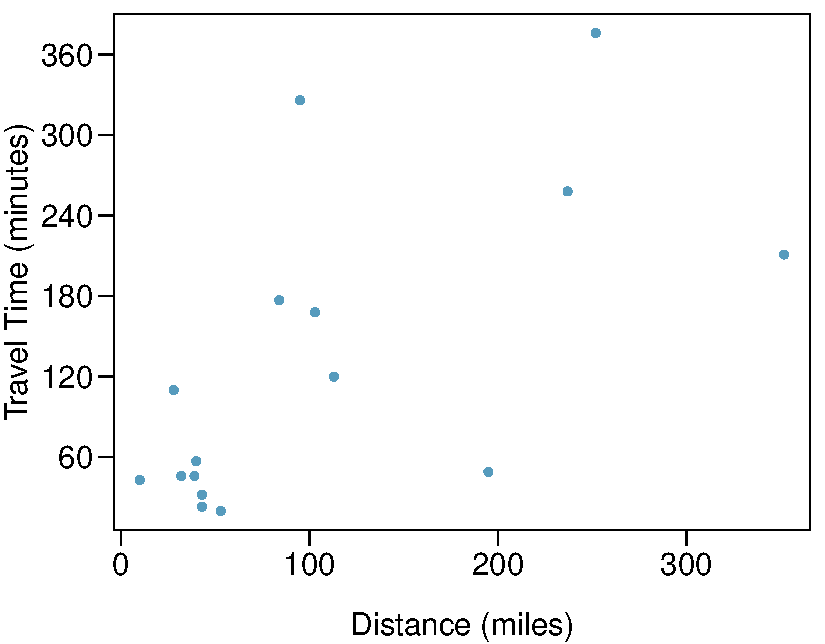
\includegraphics[width=\textwidth]{ch_regr_simple_linear/figures/eoce/coast_starlight_corr_units/coast_starlight.pdf}
\end{minipage}
}{}

% 14

\eoce{\qt{Crawling babies, Part I\label{crawling_babies_corr_units}} A study 
conducted at the University of Denver investigated whether babies take longer to 
learn to crawl in cold months, when they are often bundled in clothes that 
restrict their movement, than in warmer months.\footfullcite{Benson:1993} Infants 
born during the study year were split into twelve groups, one for each birth 
month. We consider the average crawling age of babies in each group against the 
average temperature when the babies are six months old (that's when babies often 
begin trying to crawl). Temperature is measured in degrees Fahrenheit (\degree F) 
and age is measured in weeks.\vspace{2mm}

\noindent\begin{minipage}[c]{0.4\textwidth}
\begin{parts}
\item Describe the relationship between temperature and crawling age.
\item How would the relationship change if temperature was measured in degrees 
Celsius (\degree C) and age was measured in months?
\item The correlation between temperature in \degree F and age in weeks was 
$r=-0.70$. If we converted the temperature to \degree C and age to months, what 
would the correlation be?
\end{parts} \vspace{3mm}
\end{minipage}
\begin{minipage}[c]{0.05\textwidth}
$\:$\\
\end{minipage}
\begin{minipage}[c]{0.52\textwidth}
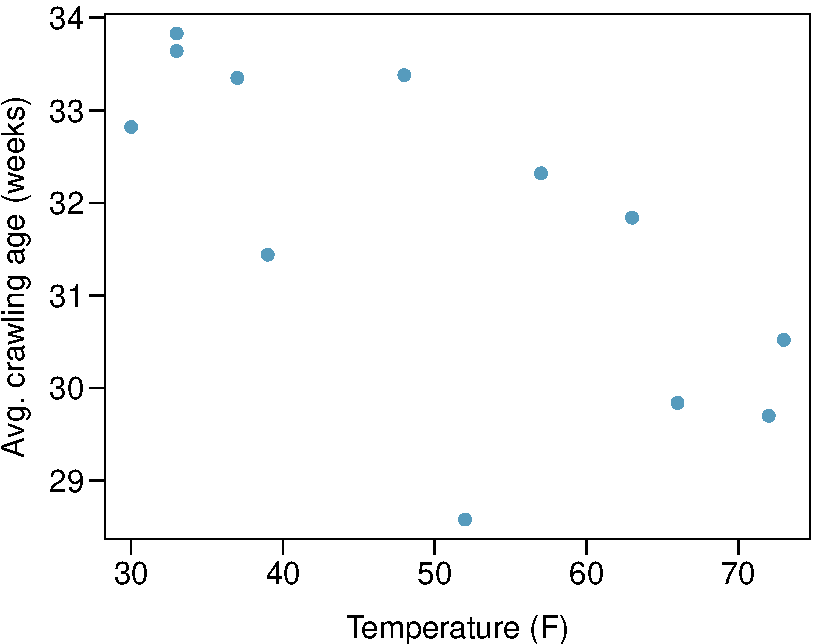
\includegraphics[width=\textwidth]{ch_regr_simple_linear/figures/eoce/crawling_babies_corr_units/crawling_babies.pdf}
\end{minipage}
}{}

% 15

\eoce{\qt{Body measurements, Part I\label{body_measurements_shoulder_height_corr_units}} 
Researchers studying anthropometry collected body girth measurements and skeletal 
diameter measurements, as well as age, weight, height and gender for 507 
physically active individuals.\footfullcite{Heinz:2003} The scatterplot below 
shows the relationship between height and shoulder girth (over deltoid muscles), 
both measured in centimeters. \\[3mm]
\begin{minipage}[c]{0.4\textwidth}
\begin{parts}
\item Describe the relationship between shoulder girth and height.
\item How would the relationship change if shoulder girth was measured in inches 
while the units of height remained in centimeters?
\end{parts}\vspace{20mm}
\end{minipage}
\begin{minipage}[c]{0.05\textwidth}
$\:$\\
\end{minipage}
\begin{minipage}[c]{0.52\textwidth}
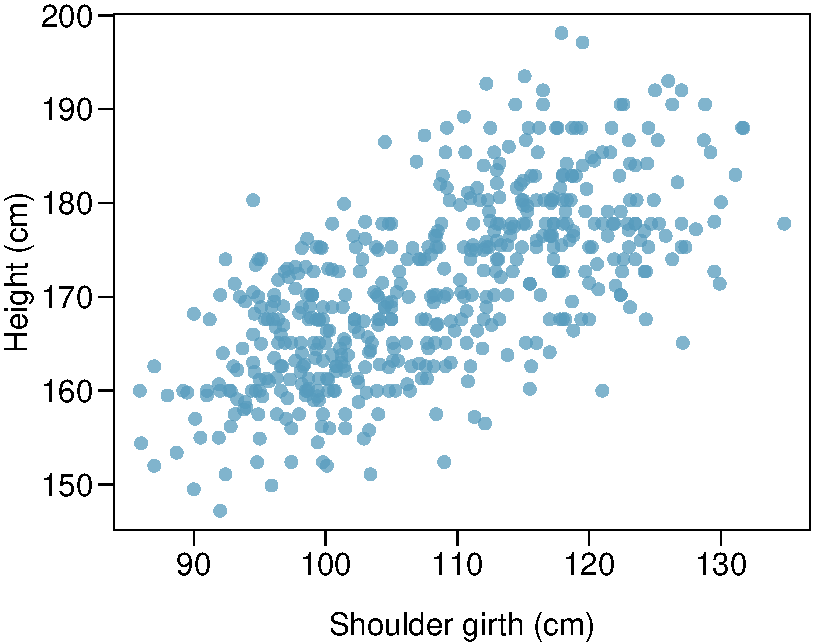
\includegraphics[width=\textwidth]{ch_regr_simple_linear/figures/eoce/body_measurements_shoulder_height_corr_units/body_measurements_height_shoulder_girth.pdf}
\end{minipage}
}{}

% 16

\eoce{\qt{Body measurements, Part II\label{body_measurements_hip_weight_corr_units}} 
The scatterplot below shows the relationship between weight measured in kilograms 
and hip girth measured in centimeters from the data described in 
Exercise~\ref{body_measurements_shoulder_height_corr_units}. \\[1mm]
\begin{minipage}[c]{0.4\textwidth}
\begin{parts}
\item Describe the relationship between hip girth and weight.
\item How would the relationship change if weight was measured in pounds while 
the units for hip girth remained in centimeters?
\end{parts}\vspace{20mm}
\end{minipage}
\begin{minipage}[c]{0.05\textwidth}
$\:$\\
\end{minipage}
\begin{minipage}[c]{0.52\textwidth}
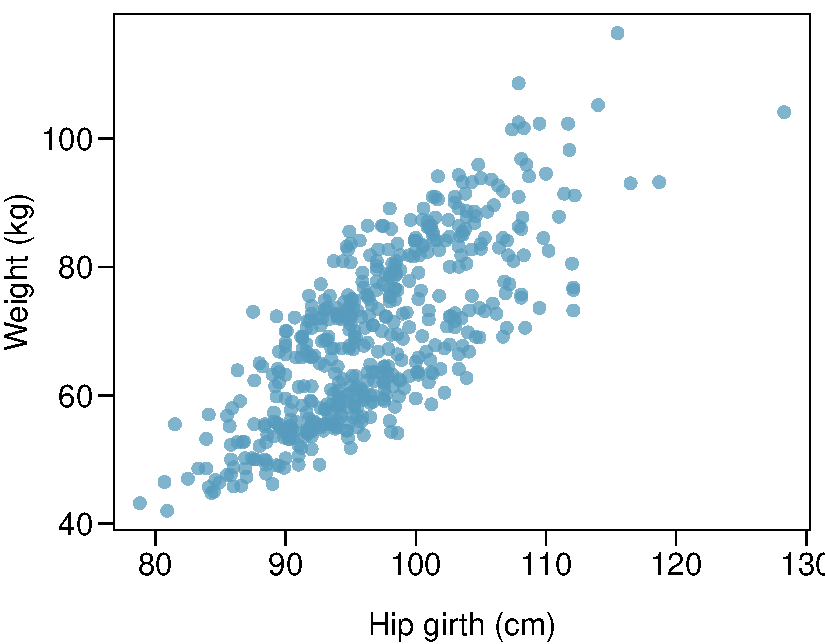
\includegraphics[width=\textwidth]{ch_regr_simple_linear/figures/eoce/body_measurements_hip_weight_corr_units/body_measurements_weight_hip_girth.pdf}
\end{minipage}
}{}

% 17

\eoce[\MarginVideo{ahss_eoce_sol-corr_husband_wife_age}]{\qt{Correlation, Part I\label{corr_husband_wife_age}} What would be the 
correlation between the ages of husbands and wives if men always married woman 
who were
\begin{parts}
\item 3 years younger than themselves? 
\item 2 years older than themselves? 
\item half as old as themselves?
\end{parts}
}{}

% 18

\eoce{\qt{Correlation, Part II\label{corr_men_women_salary}} What would be the 
correlation between the annual salaries of males and females at a company if for 
a certain type of position men always made
\begin{parts}
\item \$5,000 more than women?
\item 25\% more than women?
\item 15\% less than women?
\end{parts}
}{}


%__________________
\subsection{Fitting a line by least squares regression}

% 19
\eoce{\qt{Units of regression\label{regression_units}} Consider a regression 
predicting weight (kg) from height (cm) for a sample of adult males. What are the 
units of the correlation coefficient, the intercept, and the slope?
}{}

% 20
\eoce{\qtq{Which is higher\label{which_higher_scatter}} Determine if I or II is 
higher or if they are equal. Explain your reasoning.

\noindent For a regression line, the uncertainty associated with the slope 
estimate, $b_1$, is higher when
\begin{enumerate}
\item[I.] there is a lot of scatter around the regression line or
\item[II.] there is very little scatter around the regression line
\end{enumerate}
}{}

% 21
\eoce{\qt{Over-under, Part I\label{residual_apple_weight}} Suppose we fit a 
regression line to predict the shelf life of an apple based on its weight. For a 
particular apple, we predict the shelf life to be 4.6 days. The apple's residual 
is -0.6 days. Did we over or under estimate the shelf-life of the apple? Explain 
your reasoning.
}{}

% 22
\eoce{\qt{Over-under, Part II\label{residual_sun_cancer}} Suppose we fit a 
regression line to predict the number of incidents of skin cancer per 1,000 
people from the number of sunny days in a year. For a particular year, we predict 
the incidence of skin cancer to be 1.5 per 1,000 people, and the residual for 
this year is 0.5. Did we over or under estimate the incidence of skin cancer? 
Explain your reasoning.
}{}

% 23

\eoce{\qt{Tourism spending\label{tourism_spending_reg_conds}} The Association of 
Turkish Travel Agencies reports the number of foreign tourists visiting Turkey 
and tourist spending by year.\footfullcite{data:turkeyTourism} Three plots are 
provided: scatterplot showing the relationship between these two variables along 
with the least squares fit, residuals plot, and histogram of residuals.
\begin{center}
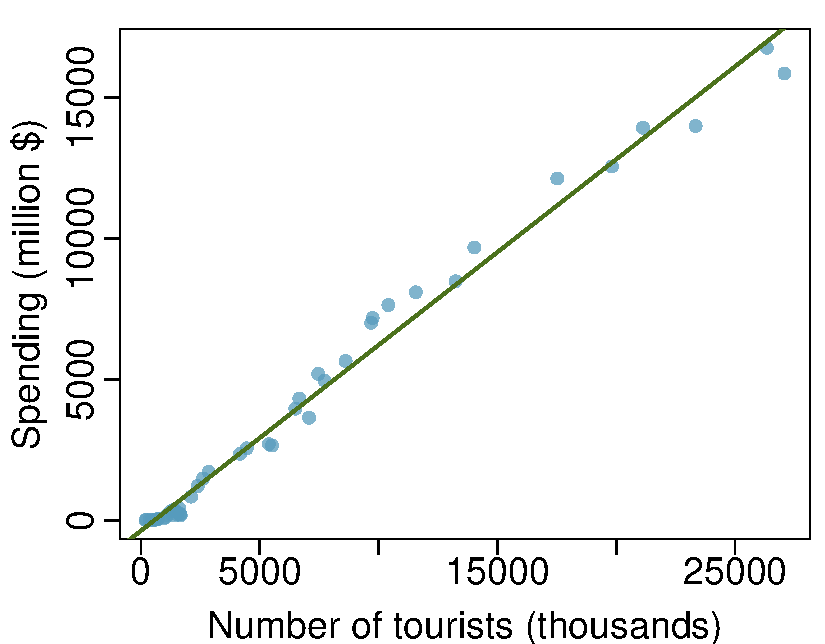
\includegraphics[width=0.32\textwidth]{ch_regr_simple_linear/figures/eoce/tourism_spending_reg_conds/tourism_spending_count.pdf}
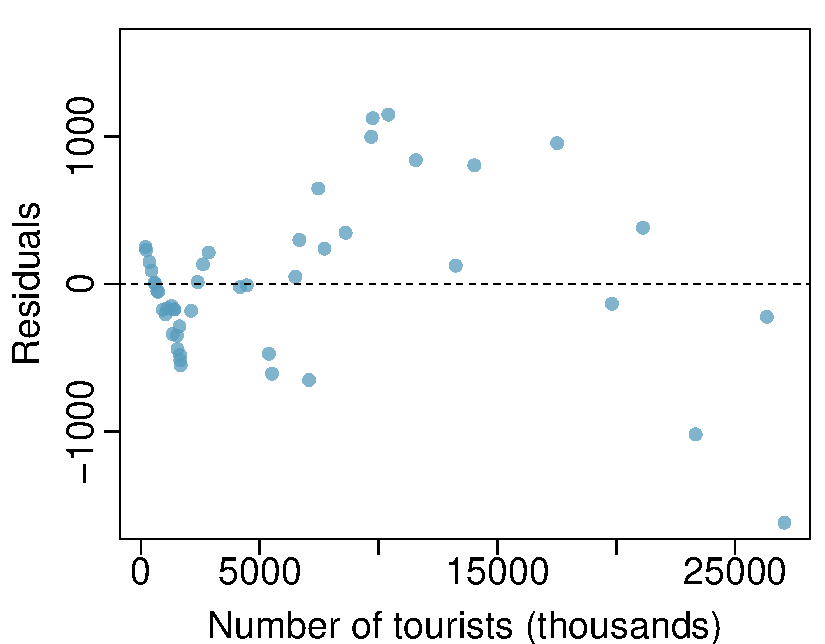
\includegraphics[width=0.32\textwidth]{ch_regr_simple_linear/figures/eoce/tourism_spending_reg_conds/tourism_spending_count_residuals.pdf}
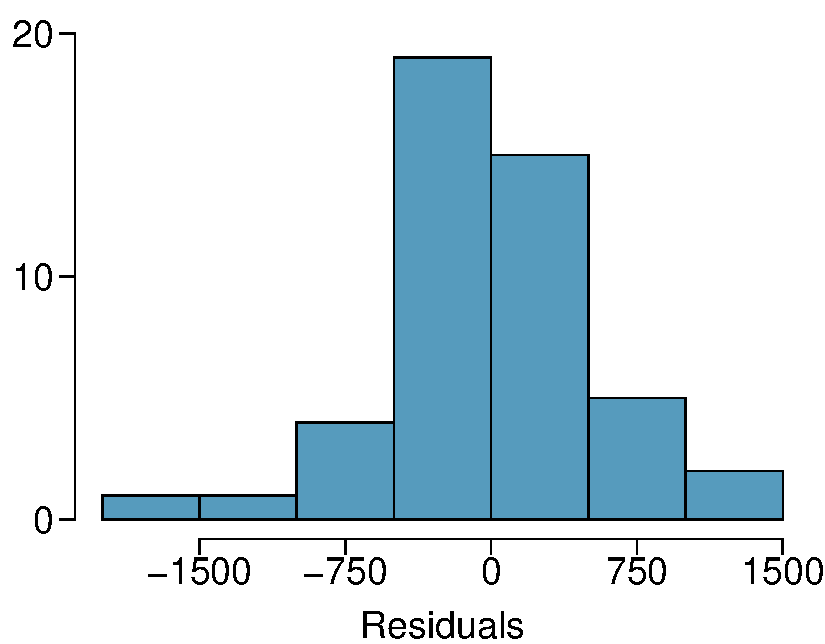
\includegraphics[width=0.32\textwidth]{ch_regr_simple_linear/figures/eoce/tourism_spending_reg_conds/tourism_spending_count_residuals_hist.pdf}
\end{center}
\begin{parts}
\item Describe the relationship between number of tourists and spending.
\item What are the explanatory and response variables?
\item Why might we want to fit a regression line to these data?
\item Do the data meet the conditions required for fitting a least squares line? 
In addition to the scatterplot, use the residual plot and histogram to answer 
this question. 
\end{parts}
}
{}

% 24

\eoce{\qt{Nutrition at Starbucks, Part I\label{starbucks_cals_carbos}} The 
scatterplot below shows the relationship between the number of calories and 
amount of carbohydrates (in grams) Starbucks food menu items 
contain.\footfullcite{data:starbucksCals} Since Starbucks only lists the number 
of calories on the display items, we are interested in predicting the amount of 
carbs a menu item has based on its calorie content.
\begin{center}
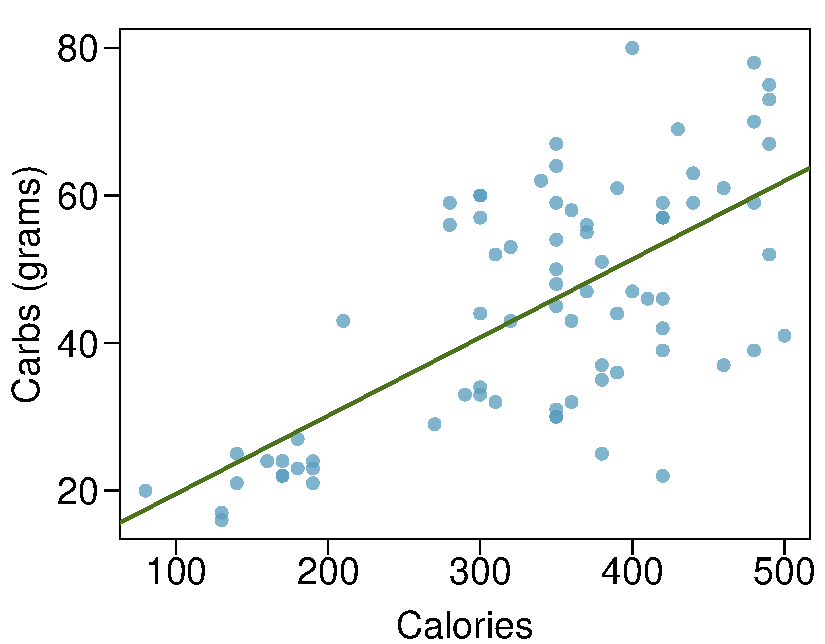
\includegraphics[width=0.32\textwidth]{ch_regr_simple_linear/figures/eoce/starbucks_cals_carbos/starbucks_cals_carbos.pdf}
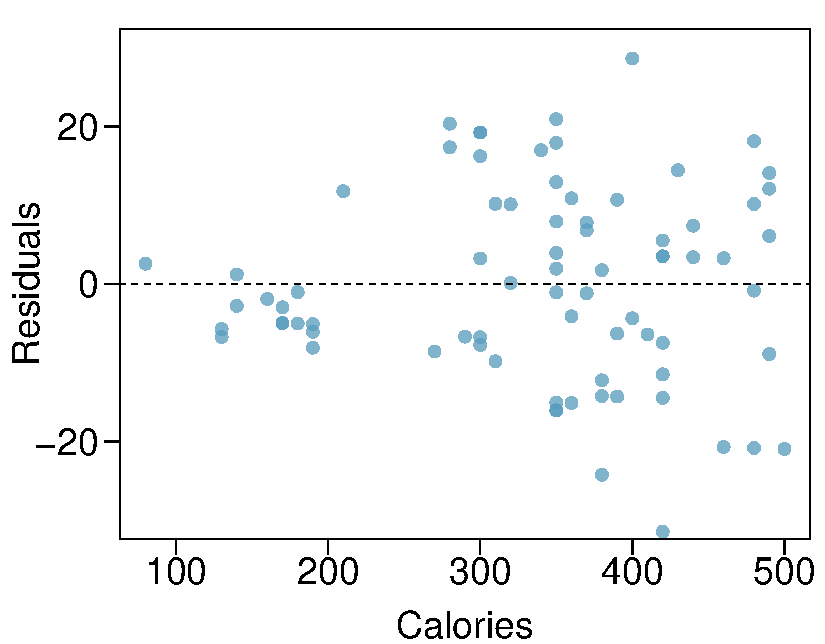
\includegraphics[width=0.32\textwidth]{ch_regr_simple_linear/figures/eoce/starbucks_cals_carbos/starbucks_cals_carbos_residuals.pdf}
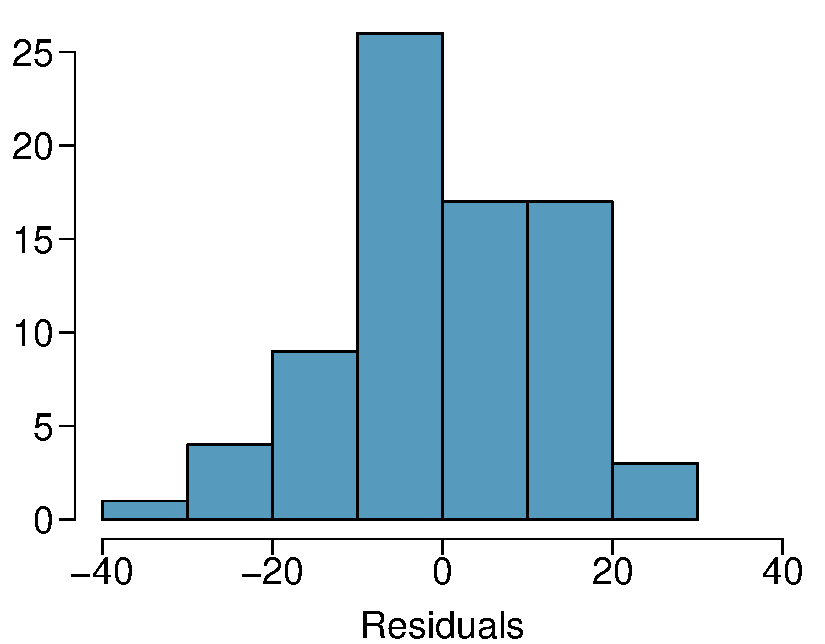
\includegraphics[width=0.32\textwidth]{ch_regr_simple_linear/figures/eoce/starbucks_cals_carbos/starbucks_cals_carbos_residuals_hist.pdf}
\end{center}
\begin{parts}
\item Describe the relationship between number of calories and amount of 
carbohydrates (in grams) that Starbucks food menu items contain.
\item In this scenario, what are the explanatory and response variables?
\item Why might we want to fit a regression line to these data?
\item Do these data meet the conditions required for fitting a least squares line?
\end{parts}
}{}

% 25

\eoce[\MarginVideo{ahss_eoce_sol-coast_starlight_reg}]{\qt{The Coast Starlight, Part II\label{coast_starlight_reg}} 
Exercise~\ref{coast_starlight_corr_units} introduces data on the Coast Starlight 
Amtrak train that runs from Seattle to Los Angeles. The mean travel time from one 
stop to the next on the Coast Starlight is 129 mins, with a standard deviation of 
113 minutes. The mean distance traveled from one stop to the next is 108 miles 
with a standard deviation of 99 miles. The correlation between travel time and 
distance is 0.636.
\begin{parts}
\item Write the equation of the regression line for predicting travel time.
\item Interpret the slope and the intercept in this context.
\item Calculate $R^2$ of the regression line for predicting travel time from 
distance traveled for the Coast Starlight, and interpret $R^2$ in the context of 
the application.
\item The distance between Santa Barbara and Los Angeles is 103 miles. Use the 
model to estimate the time it takes for the Starlight to travel between these two 
cities.
\item It actually takes the Coast Starlight about 168 mins to travel from Santa 
Barbara to Los Angeles. Calculate the residual and explain the meaning of this 
residual value.
\item Suppose Amtrak is considering adding a stop to the Coast Starlight 500 
miles away from Los Angeles. Would it be appropriate to use this linear model to 
predict the travel time from Los Angeles to this point? 
\end{parts}
}{}

% 26

\eoce{\qt{Body measurements, Part III\label{body_measurements_shoulder_height_reg}} 
Exercise~\ref{body_measurements_shoulder_height_corr_units} introduces data on 
shoulder girth and height of a group of individuals. The mean shoulder girth is 
107.20 cm with a standard deviation of 10.37 cm. The mean height is 171.14 cm 
with a standard deviation of 9.41 cm. The correlation between height and shoulder 
girth is 0.67.
\begin{parts}
\item Write the equation of the regression line for predicting height.
\item Interpret the slope and the intercept in this context.
\item Calculate $R^2$ of the regression line for predicting height from shoulder 
girth, and interpret it in the context of the application.
\item A randomly selected student from your class has a shoulder girth of 100 cm. 
Predict the height of this student using the model.
\item The student from part~(d) is 160 cm tall. Calculate the residual, and 
explain what this residual means.
\item A one year old has a shoulder girth of 56 cm. Would it be appropriate to 
use this linear model to predict the height of this child?
\end{parts}
}{}

% 27

\noindent \begin{minipage}[c]{0.56\textwidth}
\eoce{\qt{Nutrition at Starbucks, Part II\label{starbucks_cals_protein}} 
Exercise~\ref{starbucks_cals_carbos} introduced a data set on nutrition 
information on Starbucks food menu items. Based on the scatterplot and the 
residual plot provided, describe the relationship between the protein content and 
calories of these menu items, and determine if a simple linear model is 
appropriate to predict amount of protein from the number of calories.
\vspace{34mm}
}{}
\end{minipage}
\begin{minipage}[c]{0.02\textwidth}
$\:$ \\
\end{minipage}
\begin{minipage}[c]{0.4\textwidth}
\begin{center}
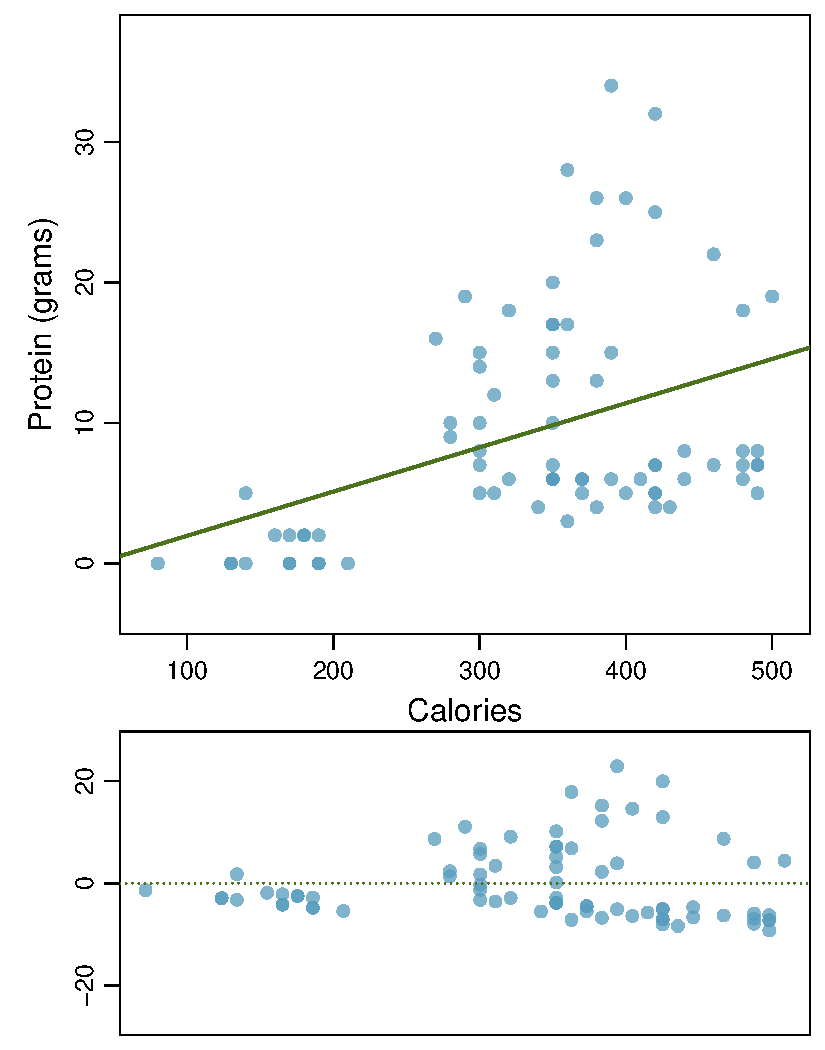
\includegraphics[width= \textwidth]{ch_regr_simple_linear/figures/eoce/starbucks_cals_protein/starbucks_cals_protein.pdf} \\
\end{center}
\end{minipage}

% 28

\eoce{\qt{Helmets and lunches\label{helmet_lunch}} 
The scatterplot shows the relationship between socioeconomic status measured as 
the percentage of children in a neighborhood receiving reduced-fee lunches at 
school ({\tt lunch}) and the percentage of bike riders in the neighborhood 
wearing helmets ({\tt helmet}). The average percentage of children receiving 
reduced-fee lunches is 30.8\% with a standard deviation of 26.7\% and the average 
percentage of bike riders wearing helmets is 38.8\% with a standard deviation of 
16.9\%.

\noindent\begin{minipage}[c]{0.55\textwidth}
\begin{parts}
\item If the $R^2$ for the least-squares regression line for these data is 
$72\%$, what is the correlation between {\tt lunch} and {\tt helmet}?
\item Calculate the slope and intercept for the least-squares regression line for 
these data.
\item Interpret the intercept of the least-squares regression line in the context 
of the application.
\item Interpret the slope of the least-squares regression line in the context of 
the application.
\item What would the value of the residual be for a neighborhood where 40\% of 
the children receive reduced-fee lunches and 40\% of the bike riders wear 
helmets? Interpret the meaning of this residual in the context of the application.
\end{parts}
\end{minipage}
\begin{minipage}[c]{0.02\textwidth}
$\:$ \\
\end{minipage}
\begin{minipage}[c]{0.43\textwidth}
\begin{center}
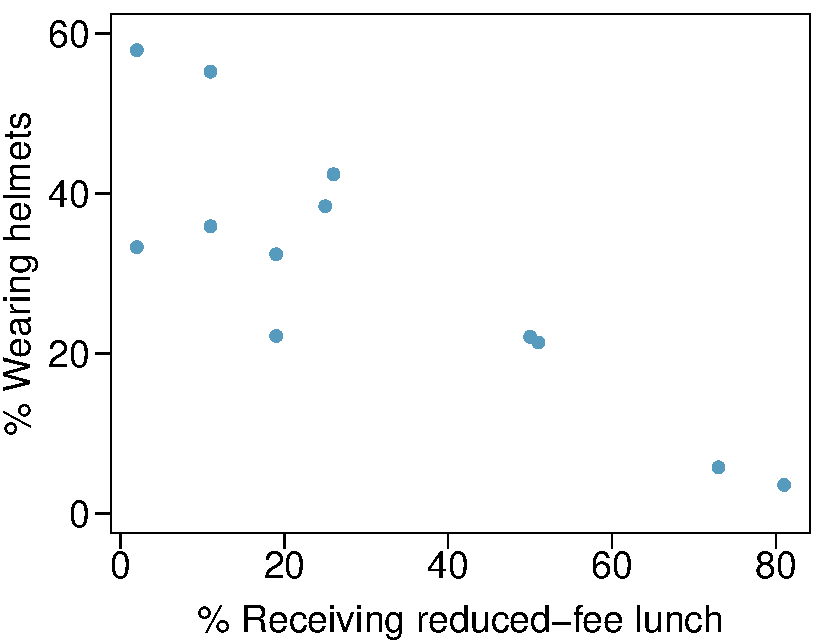
\includegraphics[width= \textwidth]{ch_regr_simple_linear/figures/eoce/helmet_lunch/helmet_lunch.pdf} \\
\end{center}
\end{minipage}
}{}

% 29

\eoce[\MarginVideo{ahss_eoce_sol-murders_poverty_reg}]{\qt{Murders and poverty, Part I\label{murders_poverty_reg}} The following 
regression output is for predicting annual murders per million from percentage 
living in poverty in a random sample of 20 metropolitan areas.\\[2mm]
\begin{minipage}[c]{0.55\textwidth}
{\small
\begin{tabular}{rrrrr}
    \hline
            & Estimate  & Std. Error    & t value   & Pr($>$$|$t$|$) \\ 
    \hline
(Intercept) & -29.901   & 7.789         & -3.839    & 0.001 \\ 
poverty\%   & 2.559     & 0.390         & 6.562     & 0.000 \\ 
   \hline
\end{tabular}
$s = 5.512 \hfill R^2 = 70.52\% \hfill R^2_{adj} = 68.89\%$ 
}
\begin{parts}
\item Write out the linear model.
\item Interpret the intercept.
\item Interpret the slope.
\item Interpret $R^2$.
\item Calculate the correlation coefficient.
\end{parts}
\end{minipage}
\begin{minipage}[c]{0.05\textwidth}
$\:$\\
\end{minipage}
\begin{minipage}[c]{0.4\textwidth}
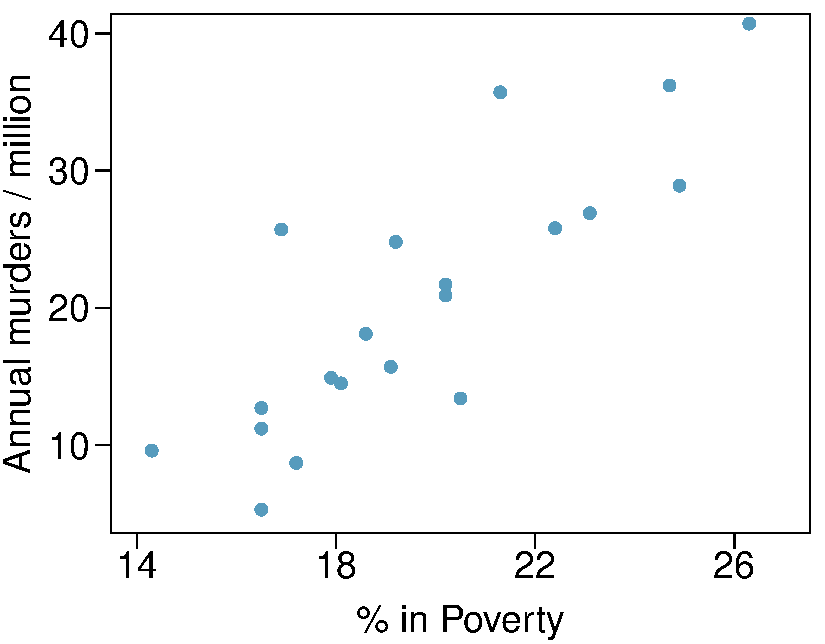
\includegraphics[width=0.99\textwidth]{ch_regr_simple_linear/figures/eoce/murders_poverty_reg/murders_poverty.pdf}
\end{minipage}
}{}

% 30

\eoce{\qt{Cats, Part I\label{cat_body_heart_reg}} The following regression output 
is for predicting the heart weight (in g) of cats from their body weight (in kg). 
The coefficients are estimated using a dataset of 144 domestic cats.\\[2mm]
\begin{minipage}[c]{0.55\textwidth}
{\small
\begin{tabular}{rrrrr}
    \hline
            & Estimate  & Std. Error    & t value   & Pr($>$$|$t$|$) \\ 
    \hline
(Intercept) & -0.357    & 0.692         & -0.515    & 0.607 \\ 
body wt     & 4.034     & 0.250         & 16.119    & 0.000 \\ 
    \hline
\end{tabular}
$s = 1.452 \hfill R^2 = 64.66\% \hfill R^2_{adj} = 64.41\%$ 
}
\begin{parts}
\item Write out the linear model.
\item Interpret the intercept.
\item Interpret the slope.
\item Interpret $R^2$.
\item Calculate the correlation coefficient.
\end{parts}
\end{minipage}
\begin{minipage}[c]{0.05\textwidth}
$\:$\\
\end{minipage}
\begin{minipage}[c]{0.4\textwidth}
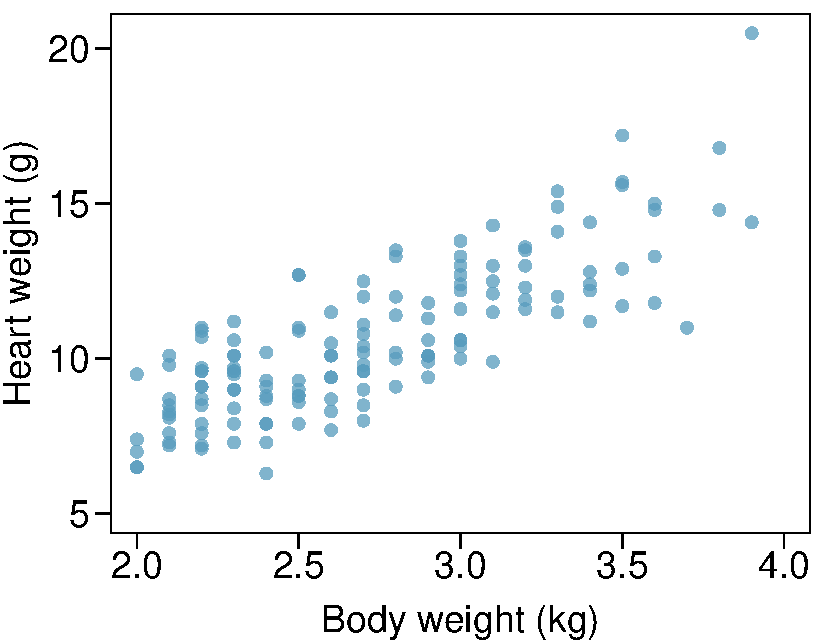
\includegraphics[width=0.99\textwidth]{ch_regr_simple_linear/figures/eoce/cat_body_heart_reg/cat_body_heart.pdf}
\end{minipage}
}{}

%__________________
\subsection{Types of outliers in linear regression}

% 31

\eoce{\qt{Outliers, Part I\label{outliers_1}} Identify the outliers in the 
scatterplots shown below, and determine what type of outliers they are. Explain 
your reasoning.
\begin{center}
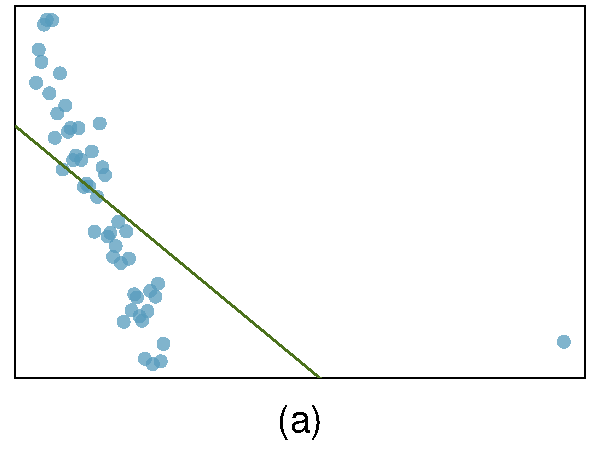
\includegraphics[width=0.32\textwidth]{ch_regr_simple_linear/figures/eoce/outliers_1/outliers_1_influential.pdf}
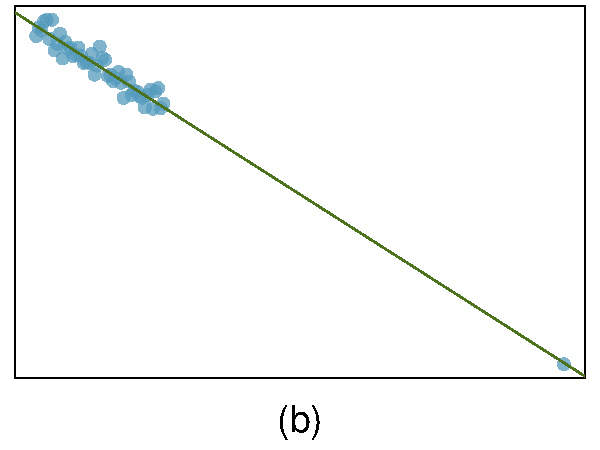
\includegraphics[width=0.32\textwidth]{ch_regr_simple_linear/figures/eoce/outliers_1/outliers_2_leverage.pdf}
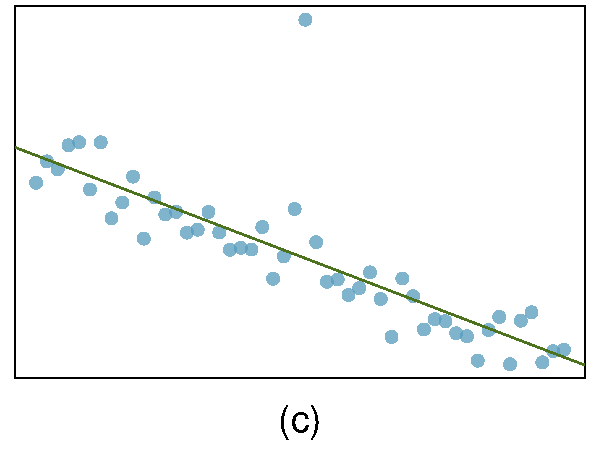
\includegraphics[width=0.32\textwidth]{ch_regr_simple_linear/figures/eoce/outliers_1/outliers_3_outlier.pdf}
\end{center}
}{}

% 32

\eoce{\qt{Outliers, Part II\label{outliers_2}} Identify the outliers in the 
scatterplots shown below and determine what type of outliers they are. Explain 
your reasoning.
\begin{center}
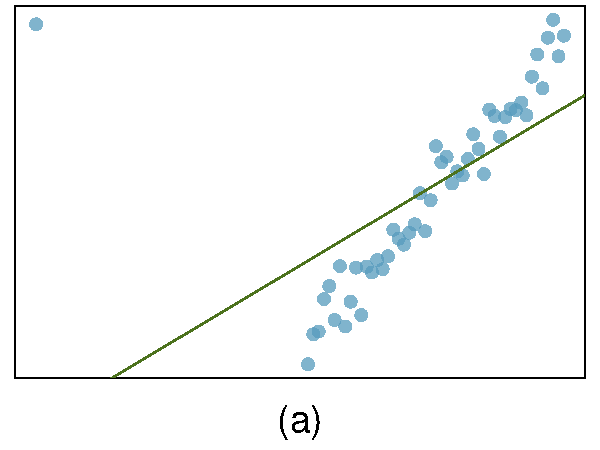
\includegraphics[width=0.32\textwidth]{ch_regr_simple_linear/figures/eoce/outliers_2/outliers_1_influential.pdf}
\includegraphics[width=0.32\textwidth]{ch_regr_simple_linear/figures/eoce/outliers_2/outliers_2_influential.pdf}
\includegraphics[width=0.32\textwidth]{ch_regr_simple_linear/figures/eoce/outliers_2/outliers_3_outlier.pdf}
\end{center}
}{}


% 33

\eoce{\qt{Urban homeowners, Part I\label{urban_homeowners_outlier}} The 
scatterplot below shows the percent of families who own their home vs. the 
percent of the population living in urban areas in 
2010.\footfullcite{data:urbanOwner} There are 52 observations, each corresponding 
to a state in the US. Puerto Rico and District of Columbia are also included.

\noindent\begin{minipage}[c]{0.5\textwidth}
\begin{parts}
\item Describe the relationship between the percent of families who own their 
home and the percent of the population living in urban areas in 2010.
\item The outlier at the bottom right corner is District of Columbia, where 100\% 
of the population is considered urban. What type of outlier is this observation?
\end{parts}
\end{minipage}
\begin{minipage}[c]{0.05\textwidth}
$\:$\\
\end{minipage}
\begin{minipage}[c]{0.4\textwidth}
\includegraphics[width=0.95\textwidth]{ch_regr_simple_linear/figures/eoce/urban_homeowners_outlier/urban_homeowners_outlier.pdf} \vspace{-3mm}
\end{minipage}
}{}

% 34

\eoce{\qt{Crawling babies, Part II\label{crawling_babies_outlier}} 
Exercise~\ref{crawling_babies_corr_units} introduces data on the average monthly 
temperature during the month babies first try to crawl (about 6 months after 
birth) and the average first crawling age for babies born in a given month. A 
scatterplot of these two variables reveals a potential outlying month when the 
average temperature is about 53\degree F and average crawling age is about 28.5 
weeks. Does this point have high leverage? Is it an influential point?
}{}


%__________________
\subsection{Inference for linear regression}

In the following exercises, visually check the conditions for fitting a least 
squares regression line, but you do not need to report these conditions in your 
solutions. \\

% 35

\eoce{\qt{Body measurements, Part IV\label{body_measurements_weight_height_inf}} The scatterplot and least squares summary below show the relationship between 
weight measured in kilograms and height measured in centimeters of 507 physically 
active individuals.

\begin{minipage}[c]{0.4\textwidth}
\begin{center}
\includegraphics[width=\textwidth]{ch_regr_simple_linear/figures/eoce/body_measurements_weight_height_inf/body_measurements_weight_height.pdf}
\end{center}
\end{minipage}
\begin{minipage}[c]{0.6\textwidth}
{\scriptsize
\begin{center}
\begin{tabular}{rrrrr}
    \hline
            & Estimate  & Std. Error    & t value   & Pr($>$$|$t$|$) \\ 
    \hline
(Intercept) & -105.0113 & 7.5394        & -13.93    & 0.0000 \\ 
height      & 1.0176    & 0.0440        & 23.13     & 0.0000 \\
    \hline
\end{tabular}
\end{center}
}
\end{minipage}
\begin{parts}
\item Describe the relationship between height and weight.
\item Write the equation of the regression line. Interpret the slope and 
intercept in context.
\item Do the data provide strong evidence that an increase in height is 
associated with an increase in weight? State the null and alternative hypotheses, 
report the p-value, and state your conclusion.
\item The correlation coefficient for height and weight is 0.72. Calculate $R^2$ 
and interpret it in context.
\end{parts}
}{}

% 36

\eoce{\qt{Beer and blood alcohol content\label{beer_blood_alcohol_inf}} Many 
people believe that gender, weight, drinking habits, and many other factors are 
much more important in predicting blood alcohol content (BAC) than simply 
considering the number of drinks a person consumed. Here we examine data from 
sixteen student volunteers at Ohio State University who each drank a randomly 
assigned number of cans of beer. These students were evenly divided between men 
and women, and they differed in weight and drinking habits. Thirty minutes later, 
a police officer measured their blood alcohol content (BAC) in grams of alcohol 
per deciliter of blood.\footfullcite{Malkevitc+Lesser:2008} The scatterplot and 
regression table summarize the findings. \\
\begin{minipage}[c]{0.4\textwidth}
\begin{center}
\includegraphics[width=0.76\textwidth]{ch_regr_simple_linear/figures/eoce/beer_blood_alcohol_inf/beer_blood_alcohol.pdf}
\end{center}
\end{minipage}
\begin{minipage}[c]{0.6\textwidth}
{\scriptsize
\begin{center}
\begin{tabular}{rrrrr}
    \hline
            & Estimate  & Std. Error    & t value   & Pr($>$$|$t$|$) \\ 
    \hline
(Intercept) & -0.0127   & 0.0126        & -1.00     & 0.3320 \\ 
beers       & 0.0180    & 0.0024        & 7.48      & 0.0000 \\ 
    \hline
\end{tabular}
\end{center}
}
\end{minipage}
\begin{parts}
\item Describe the relationship between the number of cans of beer and BAC.
\item Write the equation of the regression line. Interpret the slope and 
intercept in context.
\item Do the data provide strong evidence that drinking more cans of beer is 
associated with an increase in blood alcohol? State the null and alternative 
hypotheses, report the p-value, and state your conclusion.
\item The correlation coefficient for number of cans of beer and BAC is 0.89. 
Calculate $R^2$ and interpret it in context.
\item Suppose we visit a bar, ask people how many drinks they have had, and also 
take their BAC. Do you think the relationship between number of drinks and BAC 
would be as strong as the relationship found in the Ohio State study?
\end{parts}
}{}

% 37

\eoce{\qt{Husbands and wives, Part II\label{husbands_wives_height_inf}} The 
scatterplot below summarizes husbands' and wives' heights in a random sample of 
170 married couples in Britain, where both partners' ages are below 65 years. 
Summary output of the least squares fit for predicting wife's height from 
husband's height is also provided in the table.

\noindent\begin{minipage}[c]{0.38\textwidth}
\begin{center}
\includegraphics[width=0.8\textwidth]{ch_regr_simple_linear/figures/eoce/husbands_wives_height_inf/husbands_wives_height.pdf}
\end{center}
\end{minipage}
\begin{minipage}[c]{0.6\textwidth}
{\scriptsize
\begin{center}
\begin{tabular}{rrrrr}
    \hline
                    & Estimate  & Std. Error    & t value   & Pr($>$$|$t$|$) \\ 
    \hline
(Intercept)         & 43.5755   & 4.6842        & 9.30      & 0.0000 \\ 
height\_\hspace{0.3mm}husband   & 0.2863    & 0.0686        & 4.17      & 0.0000 \\ 
    \hline
\end{tabular}
\end{center}
}
\end{minipage}

\begin{parts}
\item Is there strong evidence that taller men marry taller women? State the 
hypotheses and include any information used to conduct the test.
\item Write the equation of the regression line for predicting wife's height from 
husband's height.
\item Interpret the slope and intercept in the context of the application.
\item Given that $R^2 = 0.09$, what is the correlation of heights in this data 
set?
\item You meet a married man from Britain who is 5'9" (69 inches). What would you 
predict his wife's height to be? How reliable is this prediction?
\item You meet another married man from Britain who is 6'7" (79 inches). Would it 
be wise to use the same linear model to predict his wife's height? Why or why not?
\end{parts}
}{}

% 38

\eoce{\qt{Husbands and wives, Part III\label{husbands_wives_age_inf}} 
Exercise~\ref{husbands_wives_height_inf} presents a scatterplot displaying the 
relationship between husbands' and wives' ages in a random sample of 170 married 
couples in Britain, where both partners' ages are below 65 years. Given below is 
summary output of the least squares fit for predicting wife's age from husband's 
age.

\begin{minipage}[c]{0.4\textwidth}
\begin{center}
\includegraphics[width=\textwidth]{ch_regr_simple_linear/figures/eoce/husbands_wives_age_inf/husbands_wives_age.pdf}
\end{center}
\end{minipage}
\begin{minipage}[c]{0.6\textwidth}
{\scriptsize
\begin{center}
\begin{tabular}{rrrrr}
  \hline
                & Estimate  & Std. Error    & t value   & Pr($>$$|$t$|$) \\ 
  \hline
(Intercept)     & 1.5740    & 1.1501        & 1.37      & 0.1730 \\ 
age\_\hspace{0.3mm}husband  & 0.9112    & 0.0259        & 35.25     & 0.0000 \\ 
   \hline
\multicolumn{5}{r}{$df = 168$} \\
\end{tabular}
\end{center}
}
\end{minipage}

\begin{parts}
\item We might wonder, is the age difference between husbands and wives 
consistent across ages? If this were the case, then the slope parameter would be 
$\beta_1 = 1$. Use the information above to evaluate if there is strong evidence 
that the difference in husband and wife ages differs for different ages.
\item Write the equation of the regression line for predicting wife's age from 
husband's age.
\item Interpret the slope and intercept in context.
\item Given that $R^2 = 0.88$, what is the correlation of ages  in this data set?
\item You meet a married man from Britain who is 55 years old. What would you 
predict his wife's age to be? How reliable is this prediction?
\item You meet another married man from Britain who is 85 years old. Would it be 
wise to use the same linear model to predict his wife's age? Explain.
\end{parts}
}{}

% 39

\eoce{\qt{Urban homeowners, Part II\label{urban_homeowners_cond}} \\
\noindent \begin{minipage}[c]{0.56\textwidth}
Exercise~\ref{urban_homeowners_outlier} gives a scatterplot displaying the 
relationship between the percent of families that own their home and the percent 
of the population living in urban areas. Below is a similar scatterplot, 
excluding District of Columbia, as well as the residuals plot. There were 51 
cases.
\begin{parts}
\item For these data, $R^2=0.28$. What is the correlation? How can you tell if it 
is positive or negative?
\item Examine the residual plot. What do you observe? Is a simple least squares 
fit appropriate for these data?
\end{parts}
\vspace{15mm}
\end{minipage}
\begin{minipage}[c]{0.02\textwidth}
$\:$ \\
\end{minipage}
\begin{minipage}[c]{0.4\textwidth}
\begin{center}
\includegraphics[width=\textwidth]{ch_regr_simple_linear/figures/eoce/urban_homeowners_cond/urban_homeowners_cond.pdf}
\end{center}
\end{minipage}
}{}

% 40

\eoce{\qt{Rate my professor\label{rate_my_prof}} Many college courses conclude by 
giving students the opportunity to evaluate the course and the instructor 
anonymously. However, the use of these student evaluations as an indicator of 
course quality and teaching effectiveness is often criticized because these 
measures may reflect the influence of non-teaching related characteristics, such 
as the physical appearance of the instructor. Researchers at University of Texas, 
Austin collected data on teaching evaluation score (higher score means better) 
and standardized beauty score (a score of 0 means average, negative score means 
below average, and a positive score means above average) for a sample of 463 
professors.\footfullcite{Hamermesh:2005} The scatterplot below shows the 
relationship between these variables, and also provided is a regression output 
for predicting teaching evaluation score from beauty score.
\noindent\begin{minipage}[c]{0.4\textwidth}
\includegraphics[width=\textwidth]{ch_regr_simple_linear/figures/eoce/rate_my_prof/rate_my_prof_eval_beauty.pdf} \\
\end{minipage}
\begin{minipage}[c]{0.6\textwidth}
\begin{tabular}{rrrrr}
    \hline
            & Estimate  & Std. Error    & t value   & Pr($>$$|$t$|$) \\ 
  \hline
(Intercept) & 4.010     & 0.0255        &   157.21  & 0.0000 \\ 
beauty      &  \fbox{\textcolor{white}{{\footnotesize Cell 1}}}  
                        & 0.0322        & 4.13      & 0.0000\vspace{0.8mm} \\ 
   \hline
\end{tabular}
\end{minipage}
\begin{parts}
\item Given that the average standardized beauty score is -0.0883 and average 
teaching evaluation score is 3.9983, calculate the slope. Alternatively, the 
slope may be computed using just the information provided in the model summary 
table.
\item Do these data provide convincing evidence that the slope of the 
relationship between teaching evaluation and beauty is positive? Explain your 
reasoning.
\item List the conditions required for linear regression and check if each one is 
satisfied for this model based on the following diagnostic plots.
\begin{center}
\includegraphics[width=0.4\textwidth]{ch_regr_simple_linear/figures/eoce/rate_my_prof/rate_my_prof_residuals.pdf}
\includegraphics[width=0.4\textwidth]{ch_regr_simple_linear/figures/eoce/rate_my_prof/rate_my_prof_residuals_hist.pdf} \\
\includegraphics[width=0.4\textwidth]{ch_regr_simple_linear/figures/eoce/rate_my_prof/rate_my_prof_residuals_qq.pdf}
\includegraphics[width=0.4\textwidth]{ch_regr_simple_linear/figures/eoce/rate_my_prof/rate_my_prof_residuals_order.pdf}
\end{center}
\end{parts}
}{}

% 41

\eoce[\MarginVideo{ahss_eoce_sol-murders_poverty_inf}]{\qt{Murders and poverty, Part II\label{murders_poverty_inf}} 
Exercise~\ref{murders_poverty_reg} presents regression output from a model for 
predicting annual murders per million from percentage living in poverty based on 
a random sample of 20 metropolitan areas. The model output is also provided below.
\begin{center}
\begin{tabular}{rrrrr}
    \hline
            & Estimate  & Std. Error    & t value   & Pr($>$$|$t$|$) \\ 
    \hline
(Intercept) & -29.901   & 7.789         & -3.839    & 0.001 \\ 
poverty\%   & 2.559     & 0.390         & 6.562     & 0.000 \\ 
    \hline
\end{tabular}
\hfill $s = 5.512 \hspace{1cm} R^2 = 70.52\% \hspace{1cm} R^2_{adj} = 68.89\%$ \hfill \\
\end{center}
\begin{parts}
\item What are the hypotheses for evaluating whether poverty percentage is a 
significant predictor of murder rate?
\item State the conclusion of the hypothesis test from part (a) in context of the 
data.
\item Calculate a 95\% confidence interval for the slope of poverty percentage, 
and interpret it in context of the data.
\item Do your results from the hypothesis test and the confidence interval agree? 
Explain.
\end{parts}
}{}

% 42

\eoce{\qt{Babies\label{babies_head_gestation_inf}} Is the gestational age (time 
between conception and birth) of a low birth-weight baby useful in predicting 
head circumference at birth? Twenty-five low birth-weight babies were studied at 
a Harvard teaching hospital; the investigators calculated the regression of head 
circumference (measured in centimeters) against gestational age (measured in 
weeks). The estimated regression line is
\[ \widehat{head\_\hspace{0.3mm}circumference} = 3.91 + 0.78 \times gestational\_\hspace{0.3mm}age \]
\begin{parts}
\item What is the predicted head circumference for a baby whose gestational age 
is 28 weeks?
\item The standard error for the coefficient of gestational age is 0.35, which is 
associated with $df=23$. Does the model provide strong evidence that gestational 
age is significantly associated with head circumference?
\end{parts} 
}{}

% 43

\eoce{\qt{Murders and poverty, Part III\label{murders_poverty_inf_one_sided}} In 
Exercises~\ref{murders_poverty_inf} you evaluated whether poverty percentage is a 
significant predictor of murder rate. How, if at all, would your answer change if 
we wanted to find out whether poverty percentage is positively associated with 
murder rate. Make sure to include the appropriate p-value for this hypothesis 
test in your answer.
}{}

% 44

\eoce{\qt{Cats, Part II\label{cat_body_heart_inf}} Exercise~\ref{cat_body_heart_reg} 
presents regression output from a model for predicting the heart weight (in g) of 
cats from their body weight (in kg). The coefficients are estimated using a 
dataset of 144 domestic cats. The model output is also provided below.
\begin{center}
\begin{tabular}{rrrrr}
    \hline
            & Estimate  & Std. Error    & t value   & Pr($>$$|$t$|$) \\ 
    \hline
(Intercept) & -0.357    & 0.692         & -0.515    & 0.607 \\ 
body wt     & 4.034     & 0.250         & 16.119    & 0.000 \\ 
    \hline
\end{tabular}
\hfill $s = 1.452 \hspace{1cm} R^2 = 64.66\% \hspace{1cm} R^2_{adj} = 64.41\%$ \hfill \\
\end{center}
\begin{parts}
\item What are the hypotheses for evaluating whether body weight is positively 
associated with heart weight in cats? 
\item State the conclusion of the hypothesis test from part (a) in context of the 
data.
\item Calculate a 95\% confidence interval for the slope of body weight, and 
interpret it in context of the data.
\item Do your results from the hypothesis test and the confidence interval agree? 
Explain.
\end{parts}
}{}
